%\documentclass[aps,prb,onecolumn,nofootinbib]{revtex4}  
\documentclass[12pt,a4paper]{article}
\usepackage[margin=1in]{geometry}  % set the margins to 1in on all sides
%\usepackage{jheppub}
\usepackage{amsmath,amsfonts,amssymb,latexsym}
\usepackage{hhline}
\usepackage{graphicx}
\usepackage[arrow,matrix]{xy}
\usepackage{tikz}
\usepackage{tikz-cd}
\definecolor{hanpurple}{rgb}{0.32, 0.09, 0.98}

\usepackage[numbers]{natbib}
\usepackage[colorlinks]{hyperref}
\hypersetup{linkcolor={hanpurple}}





\usetikzlibrary{positioning,arrows}
\usetikzlibrary{decorations.pathmorphing}
\usetikzlibrary{decorations.markings}
\newcommand{\tp}{\otimes}
\newcommand{\ra}{\rightarrow}
\newcommand{\unit}{\mathbf{1}}
\newcommand{\zz}{\mathbb{Z}}
\newcommand{\mce}{\mathcal{E}}
\newcommand{\cc}{\mathbb{C}}
\newcommand{\rr}{\mathbb{R}}
\newcommand{\mcr}{\mathcal{R}}
\newcommand{\mcz}{\mathcal{Z}}
\newcommand{\mca}{\mathcal{A}}
\newcommand{\mcd}{\mathcal{D}}
\newcommand{\mcg}{\mathcal{G}}
\newcommand{\mct}{\mathcal{T}}
\newcommand{\ul}{\underline}
\newcommand{\Mod}{\text{Mod}}
\newcommand{\Aut}{\text{Aut}}
\newcommand{\ulmcc}{\underline{\mathcal{C}}}
\newcommand{\zt}{\mathbb{Z}_2}
\newcommand{\oeo}{\text{others = 1}}
\newcommand\be            {\begin{equation}}
\newcommand\ee            {\end{equation}}
\newcommand\ba            {\begin{aligned}}
\newcommand\ea            {\end{aligned}}
\newcommand{\mcf}{\mathcal{F}}
\newcommand{\spinz}{\text{\sffamily{Z}}}
\newcommand{\spinx}{\text{\sffamily{X}}}
\newcommand{\mcl}{\mathcal{L}}
\newcommand{\mcc}{\mathcal{C}}
\newcommand{\mco}{\mathcal{O}}
\newcommand{\mcm}{\mathcal{M}}
\newcommand{\zc}{\mathcal{Z}(\mathcal{C})}
\newcommand{\id}{\text{id}}
\newcommand{\Hom}{\text{Hom}}
\newcommand{\End}{\text{End}}
\newcommand{\Tor}{\text{Tor}}
\newcommand{\Ext}{\text{Ext}}
\newcommand{\p}{\partial}
\newcommand{\wt}{\widetilde}
\usepackage{verbatim}
\newcommand{\cl}{\mathbb{C}\ell}
\newcommand{\vect}{\text{Vec}}
\newcommand{\svect}{\text{sVec}}
\newtheorem{thm}{Theorem}
\newtheorem{cor}{Corollary}
\newtheorem{lemma}{Lemma}
\newtheorem{prop}{Proposition}
\newtheorem{problem}{Problem}
\newtheorem{defn}{Definition}
\newtheorem{question}{Question}
\newcommand{\fube}{\textbf{Fube}}
\newcommand{\tube}{\textbf{Tube}}
\newcommand{\fld}{\mathcal{F}}

\newcommand{\bra}[1]{\ensuremath{\left\langle#1\right|}}
\newcommand{\ket}[1]{\ensuremath{\left|#1\right\rangle}}

\definecolor{ao(english)}{rgb}{0.0, 0.5, 0.0}
\definecolor{americanrose}{rgb}{1.0, 0.01, 0.24}
\definecolor{amber(sae/ece)}{rgb}{1.0, 0.49, 0.0}

\newcommand{\dave}[1]{{\color{ao(english)}\footnotesize{(DA) #1}}}
\newcommand{\remove}[1]{{\color{amber(sae/ece)}\footnotesize{(RM?) #1}}}

%a purple that looks different from red. EL: nice! I like the name
\definecolor{amethyst}{rgb}{0.6, 0.4, 0.8}
\newcommand{\ethan}[1]{{\color{amethyst}\footnotesize{(EL) #1}}}

\newcommand{\CapDotLeft}{\mathord{\vcenter{\hbox{
\includegraphics[scale=1]{CapDotLeft.pdf}}}}}
\newcommand{\CapDotRight}{\mathord{\vcenter{\hbox{
\includegraphics[scale=1]{CapDotRight.pdf}}}}}
\newcommand{\CupDotLeft}{\mathord{\vcenter{\hbox{
\includegraphics[scale=1,angle=180,origin=c]{CapDotRight.pdf}}}}}
\newcommand{\CupDotRight}{\mathord{\vcenter{\hbox{
\includegraphics[scale=1,angle=180,origin=c]{CapDotLeft.pdf}}}}}

\newcommand{\CupCap}{\mathord{\vcenter{\hbox{
\includegraphics[scale=1]{CupCap.pdf}}}}}
\newcommand{\CupCapDots}{\mathord{\vcenter{\hbox{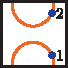
\includegraphics[scale=1]{CupCapDots.pdf}}}}}

\newcommand{\SigmaDotDot}{\mathord{\vcenter{\hbox{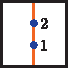
\includegraphics[scale=1]{SigmaDotDot.pdf}}}}}
\newcommand{\SigmaDotDotExchange}{\mathord{\vcenter{\hbox{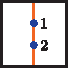
\includegraphics[scale=1]{SigmaDotDotExchange.pdf}}}}}
\newcommand{\TwoLine}{\mathord{\vcenter{\hbox{
\includegraphics[scale=1]{TwoLine.pdf}}}}}
\newcommand{\TwoLineDots}{\mathord{\vcenter{\hbox{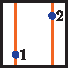
\includegraphics[scale=1]{TwoLineDots.pdf}}}}}

\newcommand{\RDotTwo}{\mathord{\vcenter{\hbox{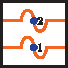
\includegraphics[scale=1]{RDotTwo.pdf}}}}}
\newcommand{\RDotTwoa}{\mathord{\vcenter{\hbox{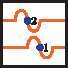
\includegraphics[scale=1]{RDotTwoa.pdf}}}}}
\newcommand{\RDotTwob}{\mathord{\vcenter{\hbox{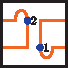
\includegraphics[scale=1]{RDotTwob.pdf}}}}}
\newcommand{\RDotTwoc}{\mathord{\vcenter{\hbox{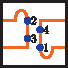
\includegraphics[scale=1]{RDotTwoc.pdf}}}}}

\newcommand{\FubeXXX}{\mathord{\vcenter{\hbox{
\includegraphics[scale=1]{EmptyTube.pdf}}}}}
\newcommand{\FubeXss}{\mathord{\vcenter{\hbox{
\includegraphics[scale=1]{OneLine.pdf}}}}}
\newcommand{\FubeXsds}{\mathord{\vcenter{\hbox{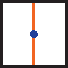
\includegraphics[scale=1]{OneLineDot.pdf}}}}}

\newcommand{\FubesXs}{\mathord{\vcenter{\hbox{
\includegraphics[scale=1,angle=90,origin=c]{OneLine.pdf}}}}}
\newcommand{\FubesdXs}{\mathord{\vcenter{\hbox{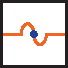
\includegraphics[scale=1]{FubesdXs.pdf}}}}}

\newcommand{\FubessX}{\mathord{\vcenter{\hbox{
\includegraphics[scale=1]{FubessX.pdf}}}}}
\newcommand{\FubessdX}{\mathord{\vcenter{\hbox{
\includegraphics[scale=1]{FubessdX.pdf}}}}}

\newcommand{\FubesXsa}{\mathord{\vcenter{\hbox{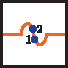
\includegraphics[scale=1]{FubesXsa.pdf}}}}}
\newcommand{\FubesXsb}{\mathord{\vcenter{\hbox{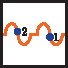
\includegraphics[scale=1]{FubesXsb.pdf}}}}}
\newcommand{\FubesXsc}{\mathord{\vcenter{\hbox{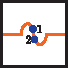
\includegraphics[scale=1]{FubesXsc.pdf}}}}}


\newcommand{\qqo}{\mathord{\vcenter{\hbox{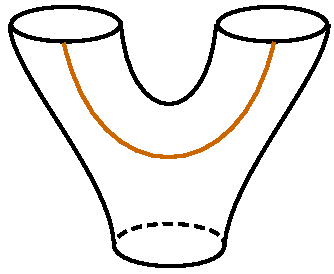
\includegraphics[scale=.4]{qq1.pdf}}}}}
\newcommand{\qtqo}{\mathord{\vcenter{\hbox{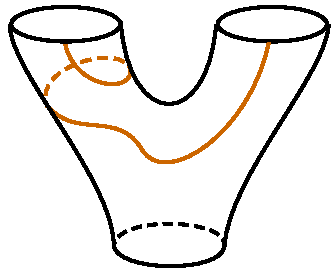
\includegraphics[scale=.4]{qtq1.pdf}}}}}
\newcommand{\qqto}{\mathord{\vcenter{\hbox{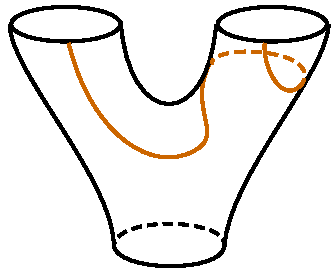
\includegraphics[scale=.4]{qqt1.pdf}}}}}
\newcommand{\qtqto}{\mathord{\vcenter{\hbox{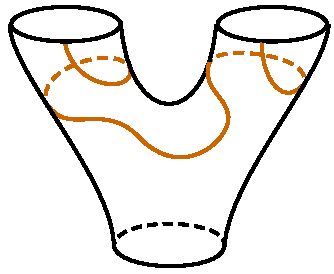
\includegraphics[scale=.4]{qtqt1.pdf}}}}}
\newcommand{\qqm}{\mathord{\vcenter{\hbox{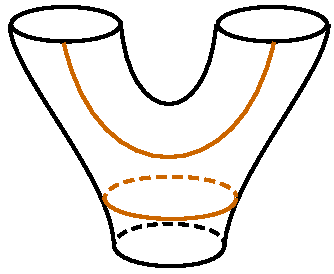
\includegraphics[scale=.4]{qqm.pdf}}}}}
\newcommand{\qtqm}{\mathord{\vcenter{\hbox{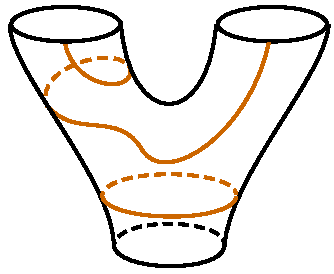
\includegraphics[scale=.4]{qtqm.pdf}}}}}
\newcommand{\qqtm}{\mathord{\vcenter{\hbox{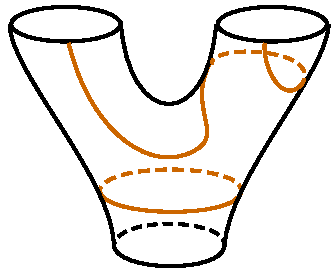
\includegraphics[scale=.4]{qqtm.pdf}}}}}
\newcommand{\qtqtm}{\mathord{\vcenter{\hbox{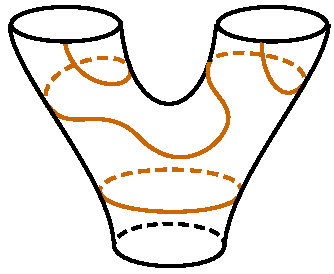
\includegraphics[scale=.4]{qtqtm.pdf}}}}}

\newcommand{\PantsPAP}{\mathord{\vcenter{\hbox{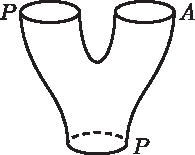
\includegraphics[scale=0.7]{PantsPAP.pdf}}}}}
\newcommand{\PantsPAsP}{\mathord{\vcenter{\hbox{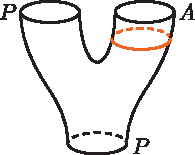
\includegraphics[scale=0.7]{PantsPAsP.pdf}}}}}

\newcommand{\PantsPsdAP}{\mathord{\vcenter{\hbox{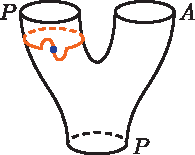
\includegraphics[scale=0.7]{PantsPsdAP.pdf}}}}}
\newcommand{\PantsPsdAsP}{\mathord{\vcenter{\hbox{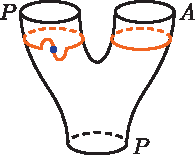
\includegraphics[scale=0.7]{PantsPsdAsP.pdf}}}}}



\newcommand{\PantsPPA}{\mathord{\vcenter{\hbox{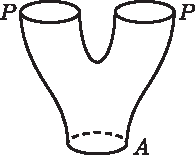
\includegraphics[scale=0.7]{PantsPPA.pdf}}}}}
\newcommand{\PantsPPAs}{\mathord{\vcenter{\hbox{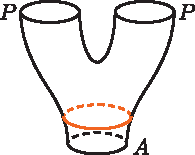
\includegraphics[scale=0.7]{PantsPPAs.pdf}}}}}

\newcommand{\PantsAsAshAsvt}{\mathord{\vcenter{\hbox{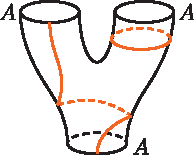
\includegraphics[scale=0.7]{PantsAsAshAsvt.pdf}}}}}
\newcommand{\PantsAstAAs}{\mathord{\vcenter{\hbox{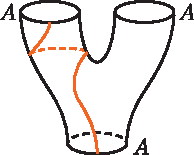
\includegraphics[scale=0.7]{PantsAstAAs.pdf}}}}}

\newcommand{\PantsAstAshAs}{\mathord{\vcenter{\hbox{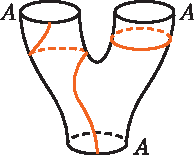
\includegraphics[scale=0.7]{PantsAstAshAs.pdf}}}}}
\newcommand{\PantsAsAshAs}{\mathord{\vcenter{\hbox{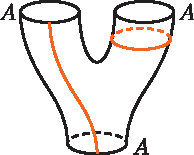
\includegraphics[scale=0.7]{PantsAsAshAs.pdf}}}}}
\newcommand{\PantsAsAAs}{\mathord{\vcenter{\hbox{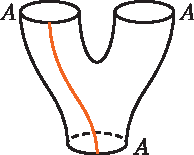
\includegraphics[scale=0.7]{PantsAsAAs.pdf}}}}}

\newcommand{\Pantssvtsvtsh}{\mathord{\vcenter{\hbox{
\includegraphics[scale=.7,origin=c]{Pantssvtsvtsh.pdf}}}}}
\newcommand{\Pantssvtsvsh}{\mathord{\vcenter{\hbox{
\includegraphics[scale=.7,angle=0,origin=c]{Pantssvtsvsh.pdf}}}}}
\newcommand{\Pantssvsvtsh}{\mathord{\vcenter{\hbox{
\includegraphics[scale=.7,angle=0,origin=c]{Pantssvsvtsh.pdf}}}}}
\newcommand{\Pantssvsvsh}{\mathord{\vcenter{\hbox{
\includegraphics[scale=.7,angle=0,origin=c]{Pantssvsvsh.pdf}}}}}
\newcommand{\PantssvtsvtX}{\mathord{\vcenter{\hbox{
\includegraphics[scale=.7,angle=0,origin=c]{PantssvtsvtX.pdf}}}}}
\newcommand{\PantssvtsvX}{\mathord{\vcenter{\hbox{
\includegraphics[scale=.7,angle=0,origin=c]{PantssvtsvX.pdf}}}}}
%\newcommand{\PantssvtsvX}{\mathord{\vcenter{\hbox{
\includegraphics[scale=.7,angle=0,origin=c]{PantssvtsvX.pdf}}}}}
\newcommand{\PantssvsvtX}{\mathord{\vcenter{\hbox{\includegraphics[scale=.7,angle=0,origin=c]{PantssvsvtX.pdf}}}}}
\newcommand{\PantssvsvX}{\mathord{\vcenter{\hbox{\includegraphics[scale=.7,angle=0,origin=c]{PantssvsvX.pdf}}}}}

\newcommand{\PantssvtXsvd}{\mathord{\vcenter{\hbox{\includegraphics[scale=.7,angle=0,origin=c]{PantssvtXsvd.pdf}}}}}
\newcommand{\Pantssvtshsvd}{\mathord{\vcenter{\hbox{\includegraphics[scale=.7,angle=0,origin=c]{Pantssvtshsvd.pdf}}}}}
\newcommand{\Pantssvshsvd}{\mathord{\vcenter{\hbox{\includegraphics[scale=.7,angle=0,origin=c]{Pantssvshsvd.pdf}}}}}
\newcommand{\PantssvXsvd}{\mathord{\vcenter{\hbox{\includegraphics[scale=.7,angle=0,origin=c]{PantssvXsvd.pdf}}}}}

\newcommand{\PantssvtXsvt}{\mathord{\vcenter{\hbox{\includegraphics[scale=.7,angle=0,origin=c]{PantssvtXsvt.pdf}}}}}
\newcommand{\PantssvXsvt}{\mathord{\vcenter{\hbox{\includegraphics[scale=.7,angle=0,origin=c]{PantssvXsvt.pdf}}}}}

\newcommand{\PantssvtXsv}{\mathord{\vcenter{\hbox{\includegraphics[scale=.7,angle=0,origin=c]{PantssvtXsv.pdf}}}}}

\newcommand{\PantssvXsv}{\mathord{\vcenter{\hbox{\includegraphics[scale=1,angle=0,origin=c]{PantssvXsv.pdf}}}}}

\newcommand{\TwoLinedotdot}{\mathord{\vcenter{\hbox{\includegraphics[scale=1.5,angle=0,origin=c]{TwoLinedotdot.pdf}}}}}

\newcommand{\Id}{\mathord{\vcenter{\hbox{\includegraphics[scale=1.5,angle=0,origin=c]{Id.pdf}}}}}

\newcommand{\CupSigmadot}{\mathord{\vcenter{\hbox{\includegraphics[scale=1.5,angle=0,origin=c]{Cupdot.pdf}}}}}

\newcommand{\CupSigma}{\mathord{\vcenter{\hbox{\includegraphics[scale=1.5,angle=0,origin=c]{Cup.pdf}}}}}

\newcommand{\StaggaredGSOdd}{\mathord{\vcenter{\hbox{\includegraphics[scale=1.5,angle=0,origin=c]{StaggaredGSOdd.pdf}}}}}
\newcommand{\StaggaredGSEven}{\mathord{\vcenter{\hbox{\includegraphics[scale=1.5,angle=0,origin=c]{StaggeredGSEven.pdf}}}}}

\newcommand{\StaggaredGSEvenR}{\mathord{\vcenter{\hbox{\reflectbox{\includegraphics[scale=1.5,angle=0,origin=c]{StaggeredGSEven.pdf}}}}}}





\newcommand{\VxsdsY}{\mathord{\vcenter{\hbox{\includegraphics[scale=0.3,angle=0,origin=c]{Vxsds.pdf}}}}}
\newcommand{\VsdxsY}{\mathord{\vcenter{\hbox{\includegraphics[scale=0.3,angle=0,origin=c]{Vsdxs.pdf}}}}}
\newcommand{\VtssdxY}{\mathord{\vcenter{\hbox{\includegraphics[scale=0.3,angle=0,origin=c]{Vtssdx.pdf}}}}}

\newcommand{\Vssdx}{\mathord{\vcenter{\hbox{\includegraphics[scale=0.3,angle=0,origin=c]{Vssdx.pdf}}}}}
\newcommand{\Vxsds}{\mathord{\vcenter{\hbox{\reflectbox{\includegraphics[scale=0.3,angle=0,origin=c]{Vssdx.pdf}}}}}}

\newcommand{\Vssx}{\mathord{\vcenter{\hbox{\includegraphics[scale=0.3,angle=0,origin=c]{Vssx.pdf}}}}}
\newcommand{\Vxss}{\mathord{\vcenter{\hbox{\reflectbox{\includegraphics[scale=0.3,angle=0,origin=c]{Vssx.pdf}}}}}}

\newcommand{\Vsxs}{\mathord{\vcenter{\hbox{\includegraphics[scale=0.3,angle=0,origin=c]{Vsxs.pdf}}}}}
\newcommand{\Vsxsd}{\mathord{\vcenter{\hbox{\includegraphics[scale=0.3,angle=0,origin=c]{Vsxsd.pdf}}}}}

\newcommand{\VsxsY}{\mathord{\vcenter{\hbox{\includegraphics[scale=0.3,angle=180,origin=c]{Vsxs.pdf}}}}}
\newcommand{\VssxY}{\mathord{\vcenter{\hbox{\includegraphics[scale=0.3,angle=180,origin=c]{Vssx.pdf}}}}}
\newcommand{\VxssY}{\mathord{\vcenter{\hbox{\reflectbox{\includegraphics[scale=0.3,angle=180,origin=c]{Vssx.pdf}}}}}}

\begin{document}


\title{First thoughts about fermions}
\author{Ethan Lake and David Aasen}
%\affiliation{Department of Physics and Astronomy, University of Utah, Salt Lake City, UT 84112, USA}
%\emailAdd{lake@physics.utah.edu}

\date{\today}

\maketitle


%\tableofcontents
\begin{abstract}
These notes are an attempt to recapitulate and elaborate on various ideaz about the process of fermion condensation in topological phases. This was motivated by Kevin Walker's IPAM talk, and after discussing some background on superfusion categories, we show how to reproduce his results for the Ising theory.
\end{abstract}

\section{Background material} 

\subsection{Supervector spaces and Clifford algebras}
 
In order to think about fermionic topological phases, it's helpful to think about the objects in tensor 
categories in terms of vector spaces. Since we're working with unitary TQFTs we will be working over $\cc$, and so the simple objects in our categories can be regarded as simple $\cc$-algebras. 

When our theories arise from fermionic degrees of freedom, the main thing we need to do is to keep track of fermion parity. We can do this by splitting all vector spaces in the theory up into a direct sum of their fermion-parity even and fermion-parity odd sectors, writing $V = V^0 \oplus V^1$. This decomposition turns vector spaces into {\it supervector} spaces, which are just $\zt$-graded versions of regular vector spaces. Throughout we will use the operator $P$ as the fermion parity operator, defined by $Pv = v$ if $v\in V^0$ (even fermion parity) and $Pv = -v $ if $v\in V^1$ (odd fermion parity). 

When we take the tensor product of two supervector spaces, we must use a super version of the tensor product which respects the $\zt$ grading. Specifically, the super version of the tensor product of two supervector spaces (which we will refer to as the tensor product, and will just denote by $\tp$) works as follows:
\be (V\tp W)^0 = V^0 \tp W^0 \oplus V^1 \tp W^1,\quad (V\tp W)^1 = V^0 \tp W^1 \oplus V^1 \tp W^0.\ee
We will use absolute value bars to denote the fermion parity of vectors in supervector spaces. That is, for $v\in V$, we write $|v| = 0$ if $Pv = v$ (i.e. if $v\in V^0$) and $|v| = 1$ if $Pv = -v$ (i.e. if $v\in V^1$). Note that since we want the $\zt$ grading to be well-defined on supervector spaces, we are forbidden from adding even fermion parity vectors with odd fermion parity vectors. 

Since we're working with a tensor product that respects the fermion parity structure of supervector spaces, it must account for the factors of $(-1)$ that appear when the relative order of two fermionic vectors in a tensor product is switched. This means that the tensor product of two vectors is supercommutative, in the sense that the wedge product is supercommutative:
\be v\tp w = (-1)^{|v||w|}w\tp v.\ee
This means that sVec (the category of supervector spaces, containing just the vacuum and a fermion) naturally comes equipped with the structure of a braided category, with the supercommutative nature of the tensor product controlling the $-1$ braiding of the fermion with itself. 

%\dave{I found this confusing. The entire category doesn't need to have a braided structure, does it? Are you just saying that the fermionic dof have a braided structure?} \ethan{Yeah, that's correct. sVec is literally just the category whose simple objects are 1 and $\psi$ -- the point is that this is automatically braided, since the definition of a supervector space allows us to define a braiding between fermionic vectors. Of course, this braided structure on sVec can be embedded into the braided structure of the ``fermionic vacuum'' of more complicated theories.  }

If a supervector space $V$ has $\dim V^0 = a$ and $\dim V^1 = b$, we say that $V$ has superdimension $a|b$. We will use the notation $\cc^{a|b}$ to denote the supervector space of superdimension $a|b$, so that $\cc^{a|b}$ is an $(a+b)$-dimensional vector space with $a$ fermion-parity even generators and $b$ fermion-parity odd generators. 

When we tensor $\cc^{a|b}$ with $\cc^{c|d}$, the graded dimensions behave in the same way that supervector spaces behave when you tensor them together. That is, they behave just like you would expect: 
\be  \cc^{a|b}\tp \cc^{c|d} \cong \cc^{ac + bd | ad + bc}.\ee
Notice in particular that $\cc^{a|b} \tp \cc^{1|0} \cong \cc^{a|b}$ and $\cc^{a|b} \tp \cc^{0|1} \cong \cc^{b|a}$. That is, tensoring with $\cc^{1|0} = \cc$ does nothing (as it should), and tensoring with $\cc^{0|1}$ is equivalent to flipping fermion parity. 

The supervector space $\cc^{1|1}$ will turn out to play an important role in what follows. This is because it is invariant under fermion-parity flips: $\cc^{1|1} \tp \cc^{0|1} \cong \cc^{1|1}$. It is also an example of a Clifford algebra, namely the Clifford algebra $\cl_1$. Clifford algebras will be important for us when we consider theories with Majoranas, and so we will quickly review their definition and basic properties. 
%\dave{Is it true that they show up anytime a fermion is around, or is it only when Majorana-type fermions are around?}\ethan{yep you're right, only when Majoranas are around. Not sure what I was thinking when I wrote that. One could argue that they always show up becuase spin structures are determined by Clifford algebras (e.g, the Spin(n) groups are really just Clifford algebras), but this isn't important for us.}

The complex Clifford algebras $\cl_n$ are the supervector spaces generated by the number 1 and $n$ {\it parity-odd} generators $\gamma_1,\dots,\gamma_n$ which satisfy the relations 
\be \{\gamma_i,\gamma_j\} = 2Q_{ij},\ee
where $\{\gamma_i,\gamma_j\} = \gamma_i\tp \gamma_j + \gamma_j\tp\gamma_i$ and $Q_{ij}$ is some quadratic form. For real Clifford algebras $Q_{ij}$ can generically be written as a diagonal matrix with $\pm1$s on the diagonal, although our working over $\cc$ allows us to set $Q_{ij} =\delta_{ij}$ without loss of generality.

The simplest (other than $\cl_0 = \cc$) Clifford algebra is $\cl_1 = \langle 1, \gamma\rangle$, with $\gamma^2 = 1$ and $P\gamma = -\gamma$. 
Since by definition $\cl_1$ has one even generator ($1$) and one odd generator ($\gamma$), we have $\cl_1 \cong \cc^{1|1}$. In terms of representations, we can choose a representation $\rho$ such that $\rho(1) = \unit_{2\times 2}$ and $\rho(\gamma) = \sigma^x$, which is consistent since $\{\sigma^x,\sigma^x\} = 2\unit_{2\times2}$ and $\sigma^x : \cc^{1|0} \mapsto \cc^{0|1}, \cc^{0|1}\mapsto \cc^{1|0}$, $i.e.$ $\sigma^x$ is odd. We will see that $\cl_1$ is the prototypical ``Majorana'' supervector space that will appear later on.

We will need a few miscellaeous facts about Clifford algebras, which we will list off here. First, tensoring two Clifford algebras gives a larger Clifford algebra whose associated quadratic form is the direct sum of the quadractic forms of the smaller algebras, meaning that the larger Clifford algebras can be built from $\cl_1$ as $\cl_n \cong \cl_1^{\tp n}$. Secondly, $\cl_2 \cong \End(\cc^{1|1})$, and since the endomorphism rings of matrix algebras always have trivial modules, $\cl_2$ and $\cc$ are Morita equivalent (written $\cl_2 \cong_M \cc$), meaning that their simple modules are the same. This will be of use later when we look at constructing quasiparticles and their fusion rules. Since $\cl_n \cong \cl_1^{\tp n}$, this implies the $\cl_n \cong_M \cl_{n+1}$ of Bott periodicity fame. % We can see this by choosing the representation $\rho(1) = \unit_{2\times2},\rho(\gamma_1)=\sigma^x,\rho(\gamma_2)=\sigma^y$. 


\begin{comment}
\subsection{Modules and Morita equivalence}\label{sec:morita}
\remove{A module over an algebra is a vector space whose scalars are drawn from the algebra. That is, it's a way of giving an algebra an action on a vector space. So modules are the algebra analogue of representations: representations construct a way for groups to act on vector spaces, and modules do the same thing for algebras. 

A mathematical concept that will be relevant is the notion of {\it Morita equivalence}. Roughly, Morita equivalence is a way of establishing when two algebras ``have the same modules'', or when their ``representation theory is the same''. The technical definition is that two algebras $A$ and $B$ are Morita equivalent (written $A\cong_M B$) when the cateogries of their left modules Mod$^L(A)$ and Mod$^L(B)$ are equivalent, although we won't use this definition much. 

The reason why the notion of Morita equivalence is useful for us is because quasiparticles in topological phases are identified with simple modules of an algebra $\fube$ called the {\it Fube algebra}, which we'll talk about in more detail later. Usually figuring out the algebra structure of \fube\ is straightforward, although computing its simple modules (aka finding an idempotent decomposition of \fube) can \remove{often} be \remove{a huge pain} tedious. Since Morita equivalent algebras have the same modules, we can often replace a complicated fube algebra or a sub-algebra of a fube algebra with a much simpler but Morita equivalent algebra, which can greatly facilitate the determination of its simple modules.

The canonical example of Morita equivalent algebras are the matrix algebras. It turns out that we actually have $\cc(n) \cong_M \cc$ for all $n$ (where $\cc(n)$ are complex $n\times n$ matrices). \dave{Is this the statement that the only thing that commutes with all $\cc(n)$ is $\cc \times  1_{n\times n}$?} \ethan{Not exactly the same as far as I know, but the fact that $Z(\cc(n)) \cong \cc$ is a necessary condition for the Morita equivalence between $\cc(n)$ and $\cc$. In general, if two algebras are Morita equivalent then their centers must be the same, but I don't think the converse holds in general (can't think of a counterexample off the top of my head though.}  This can be seen by using the following proposition:

\begin{prop}
Let $A,B$ be two algebras, and $\mce$ be an $A-B$ bimodule, that is, let $\mce$ be a left $A$-module and a right $B$-module. Suppose $\mce$ is such that 
\be \mce^* \tp_A \mce \cong B,\qquad \mce\tp_B \mce^* \cong A.\ee
Then $A$ and $B$ are Morita equivalent.
\end{prop}
We will do the proof by setting up the equivalence between the modules of $A$ and $B$ explicitly. Suppose $M$ is a module over $A$, and $N$ a module over $B$. Construct the functors $F : \Mod(A) \ra \Mod(B)$, $G:\Mod(B) \ra \Mod(A)$ as
\be F: M \mapsto \Hom_A(\mce,M),\qquad G : N \mapsto \mce\tp_B N.\ee
This associates $M$ with a $B$-module and $N$ with an $A$-module. We claim that this is an isomorphism, namely that $F$ and $G$ are inverses of one another. If this is true, we must have 
\be M \cong \mce\tp_B \Hom_A(\mce,M) \cong (\mce \tp_B \mce^*)\tp_A M,\qquad N\cong \Hom_A(\mce,\mce\tp_B N)\cong (\mce^*\tp_A\mce)\tp_BN,\ee
but this holds precisely due to our assumptions on $\mce\ \square$. 

The Morita equivalence between $\cc(n)$ and $\cc$ then follows from setting the bimodule $\mce$ to be $\mce = \cc^n$ in the above construction. 

As a useful nonexample, $\cc^n \not\cong_M \cc^m$ for any $n\neq m$. This can be seen by realizing that the centers of two Morita equivalent algebras must always be the same. This is true for the $\cc(n) \cong_M \cc$ example considered above, but of course the centers of $\cc^n$ and $\cc^m$ are different if $n\neq m$, and so indeed $\cc^n \not\cong_M \cc^m$. 

One useful fact that we will exploit in calculations is that two algebras $A$ and $B$ are always Morita equivalent if there exists a supervector space $V$ such that 
\be A \cong B \tp_\cc \End(V).\ee

For a useful example of this, we turn to the Clifford algebras. We will use the fact that  \be\cl_2 \cong \End(\cl_1) \cong \End(\cc^{1|1}),\ee
which can be seen just by realizing that $\End(\cl_1) \cong \cl_1 \tp \cl_1 \cong \cl_2$. This means that 
\be \cl_{n+2} \cong_M \cl_n\ee
for all $n$, and so $\cl_{n+2}$ and $\cl_n$ always have the same modules (this is Bott periodicity!). In particular, we see that $\cl_2$ has the same modules as $\cc$! This will be very helpful later on when we look at condensing fermions in the Ising theory. There, we will run into subalgebras of \fube\ that are isomorphic to $\End(\cc^{1|1})$. By what we've just seen these subalgebras must have the same modules as $\cc$, which is much easier to work with than $\cl_2$. Since the modules of the \fube\ algebra (and its subalgebras) determine the quasiparticles in the theory, which see in particular that subalgebras of \fube\ given by $\End(\cc^{1|1})$ must give rise to only a single quasiparticle, since we are free to replace them by the trivial algebra $\cc$.  }
\end{comment}


\section{Superfusion categories} 


When we go from fusion categories to superfusion categories, the simple objects become associated with supervector spaces, and understanding what happens to them is fairly straightforward. 
However, the fusion spaces also become superspaces, which for us is very important. In particular, this means that all the Hom spaces ($a.k.a$ fusion spaces) carry a $\zt$-grading that keeps track of their fermion parity. In particular, $\Hom_\mcc(X,Y)^0$ contains all the morphisms between $X$ and $Y$ that are fermion-parity even, and $\Hom_\mcc(X,Y)^1$ contains all the morphisms that are fermion-parity odd. So, we can think of $\Hom(X,Y)^0$ as being a regular ``bosonic'' fusion space, while $\Hom(X,Y)^1$ is an odd fusion space in which the fermion parity of the fusion products changes sign. Because of this, we can think of fusion spaces with odd fermion parity as localizing a fermion that lives on the fusion vertex. Especially important for us will be the case when our theories come with objects $X$ such that $\Hom(X,X)^1$ is nontrivial. These objects will be ``Majorana'' in some sense, and we will discuss them in more detail later. 
%\dave{Why isn't $\Hom_\mcc(X,Y)^0$ the space of homomorphisms that take even generators to even, and odd to odd? and the oppisote for $\Hom_\mcc(X,Y)^1$? It would be cool to have some intuition for this definition. Did you get it from Usher? Maybe we should also be adding references..} \ethan{You're right about the Hom spaces, and that's essentially what I wrote. Tried to fix the definition a bit. Not sure where it was from, but references might be good in any case.} 
For any morphism $f : X\ra Y$, we will write the parity of $f$ as $|f| = 
0$ if $f$ is even (preserves fermion parity) and $|f| = 1$ if $f$ is odd (reverses fermion parity). 

Without loss of generality, we can consider fusion diagrams built from a tensor product of fusion spaces of the form $\Hom(X\tp Y,Z)$. Forming a fusion graph requires choosing basis vectors for all these fusion spaces. Following convention, we will write $s^{XY}_Z(\alpha)$ to denote the parity of the basis vector for the fusion space $\Hom(X\tp Y,Z)$, where $1\leq\alpha\leq N^{XY}_Z$. For notational simplicity we will initally assume $N^{XY}_Z \leq 1$, so that all the fusion spaces are one-dimensional and have a unique fermion parity (although some of the Fibonacci-like theories we will want to consider later won't satisfy this restriction). 

The grading of morphisms is important to keep track of, since morphisms satisfy their own supercommutativity law, called the {\it superexchange law}, which states that for any four morphisms $f,g,h,k \in \mcc$, we have
\be (f\tp g) \circ (h\tp k) = (-1)^{|g||h|}(f\circ g)\tp(g\circ k).\ee
Let's run through how to see this. First of all, recall that in normal fusion categories, the tensor product of two morphisms is the same as horizontal superposition:
\be \includegraphics{ftpg.pdf}\ee
In {\it superfusion} categories, we need to be more careful, since morphisms (like the guys in the $\Hom(X\tp Y,Z)$ fusion spaces) can carry nontrivial fermion parity. This means that if we place two odd morphisms side-by-side, the relative positions of the fermions they harbor is ambiguous. This ambiguity is actually really easy to fix diagrammatically: we just write the tensor product of two morphisms in a displaced way, where the first morphism in the tensor product is displaced above the second:
\be \includegraphics{superftpg.pdf} \ee


Moving two morphisms past each other vertically may then result in a minus sign, since if both morphisms have odd fermion parity, moving them past each other is like exchanging two fermions. That is, 
\be \includegraphics{morphism_commutativity.pdf}\ee
With this property, it becomes easy to verify the superexchange law. 



%The most important morphisms we'll be grading are the fusion spaces present in fusion diagrams. Since we assume that all the nonzero fusion spaces to be one-dimensional, we can let $H^{XY}_Z$ denote the basis vector of the space $\Hom(X\tp Y,Z)$, so that $|H^{XY}_Z| = s^{XY}_Z$. 


Finally, let's quickly mention the $F$-moves (we'll come back to them in more detail later). Recall that we can write them as the basis changes
\be [F^{ijk}_l] : \bigoplus_m \Hom(i\tp j,m) \tp \Hom(m\tp k,l) \cong \bigoplus_n \Hom(i\tp n,l) \tp \Hom(j\tp k,n).\ee
The $F$-moves shouldn't change the fermion parity of the fusion graph, and so must be {\it even} morphisms. This means that the fermion parity on both sides of the above isomorphism must be the same. To quantify this condition, the even-ness of $F$ means that 
\be \label{scond}  s^{ij}_m + s^{mk}_l = s^{jk}_n + s^{in}_l,\ee
where $s^{ij}_m$ is the parity of the fusion space $\Hom(i\tp j,m)$ as before.
In particular, if $\mcc = \vect_G$ for some finite Abelian $G$, this is equivalent to the 2-cocycle condition, and so we see that such theories are (partially) classified by a choice of cohomology class $s \in H^2(BG,\zt)$. 

\subsection{Categorical caveats}\label{sec:ccs}
A number of formulae that we're used to using when working with fusion categories fail to hold upon passing to superfusion categories, while others go through unchanged. 
\begin{comment}
First, direct sums in superfusion categories factor out of $\Hom$s in the usual way:
\be \Hom(\bigoplus_i X_i,Y) \cong \bigoplus_i\Hom(X_i,Y),\qquad \Hom(X,\bigoplus_i Y_i) \cong \bigoplus_i\Hom(X,Y_i) .\ee
This happens in any (graded or otherwise) fusion category that we can cook up (at least provided we work with finitely many objects).\end{comment} 

The most important thing that needs to be modified is the way we write resolutions of the identity. Consider the usual ``coproduct'' isomorphism
\be\label{copiso} \Hom(X,Y) \cong \bigoplus_{Z\in \mcc} \Hom(X,Z) \tp \Hom(Z,Y).\ee
This amounts to stitching $X$ and $Y$ together by summing over all the simple objects that can connect $X$ to $Y$. 
\begin{comment} To put it in other words, consider the diagram
\be
\begin{tikzcd}
X \arrow[r] \arrow[dr, dashrightarrow]
& Z \arrow[d]\\
& Y
\end{tikzcd}
\ee
The isomorphism \eqref{copiso} says that going along the dashed arrow is equivalent to the sum of all the different ways to go along the two-arrow path \dave{I would have thought that the commutative diagram needs a sum over $Z$ or something. But you know better than me. } \ethan{no, you're correct, I just wrote ``sum over all ways to go along the two-arrow path'' to mean an implicit summation over $Z$, because I'm bad at writing. I vote to get rid of the diagram though -- not saying anything that the other things don't}. 
\end{comment}

In string-net diagrams, we usually see \eqref{copiso} used to write the resolution of the identity 
\be \Hom(X\tp Y,X\tp Y) \cong \bigoplus_{Z\in \mcc} \Hom(X\tp Y,Z) \tp \Hom(Z,X\tp Y),\ee
where $X,Y,$ and $Z$ are all simple objects. Diagrammatically, this looks like 
%\be \includegraphics{resid.pdf} \ee


However, these isomorphisms do not hold as written in more general settings, namely when the simple objects fail to all possess trivial endomorphism algebras. In this scenario, the RHS of \eqref{copiso} will be much bigger than the left, since the ``internal'' degrees of freedom $Z$ may contribute nontrivially to the size of the RHS.
If not all the objects have trivial endomorphism algebras, the big direct sum on the RHS of \eqref{copiso} needs to be replaced with a colimit, although we won't need to go into any detail about what this means mathematically. %Also note that as a corollary of this, $\End(X) \tp \End(Y)\not\cong\End(X\tp Y)$ in general.

The simple way to fix \eqref{copiso} involves changing the type of tensor product we use. Until now, we've tacitly been assuming that all of our tensor products are secretly $\tp_\cc$, tensor products over $\cc$. This works only when we're working in ``regular'' categories, where the Hilbert spaces associated with worldlines are always $\cc$. However, we run into problems if we have objects with $\End(Z) \not\cong \cc$ and continue to use $\tp_\cc$. If $\End(Z)$ is bigger than $\cc$, then the RHS of \eqref{copiso} is bigger than the LHS, since the internal $Z$ leg of the fusion diagram contributes a larger space to the direct sum. This is unphysical though, since the internal worldlines of freedom $Z$ shouldn't carry any more information than is carried by the incoming and outgoing worldlines (since if this were the case, the sizes of the Hilbert spaces of fusion diagrams would blow up). 

We can fix this issue by ``modding out'' by the Hilbert spaces of the internal worldlines. 
This can be done by treating $\End(Z)$ as the tensor unit when we tensor the two fusion spaces in \eqref{copiso} together. The correct formula is then
\be  \Hom(X,Y) \cong \bigoplus_{Z\in \mcc} \Hom(X,Z) \tp_{\End(Z)} \Hom(Z,Y).\ee
As a corollary, this means that the superfusion $F$-symbols should be written as 
\be [F^{ijk}_l] : \bigoplus_m \Hom(i\tp j,m) \tp_{\End(m)} \Hom(m\tp k,l) \cong \bigoplus_n \Hom(i\tp n,l) \tp_{\End(n)} \Hom(j\tp k,n).\ee
%Note that the tensor products inside the Homs are still understood as $\tp_\cc$ (should do a good job of justifying this). 

Finally, on another cautionary note, we should really be writing $\Hom_\mcc(X)$, just to distinguish it from $\Hom_\cc(X)$, and likewise for $\End_\mcc$. Let's focus on $\End_\mcc(X)$. $\End_\mcc(X)$ is the space of all endomorphisms of $X$ that {\it respect the structure of the category $\mcc$}. For example, if $\mcc = {\rm Rep}(G)$, $\End_\mcc(X)$ is the space of morphisms that commute with the $G$-action. This is very different from the more familiar (and much larger!) space of all $\cc$-linear maps from $X$ to itself, which is $\End_\cc(X)$. In particular, we have the familiar $\End_\cc(X) \cong X^*\tp X$, but this definitely doesn't hold for $\End_\mcc(X)$! Likewise, $X^*$ is certainly not defined by $\Hom_\mcc(X,\cc)$. Instead, we can define $X^*$ through 
\be \Hom_\mcc(Y,X\tp Z) \cong \Hom_\mcc(X^*\tp Y,Z).\ee
Of course, all Hom spaces should be understood as Hom$_\mcc$ spaces unless stated otherwise. 

 
\subsection{Majorana objects}

We might naively think that fusing a physical fermion with a worldline $X$, which corresponds to 
doing $X \tp \cc^{0|1}$, would always be an odd morphism on $X$. That is, we might guess that 
doing $X\tp \cc^{0|1}$ would always change the grading (fermion parity) of $X$. However, this may not always 
be true! Adding a fermion can actually be an even operation, provided that $X$ worldlines are left invariant after tensoring with $\cc^{0|1}$. This happens precisely when 
\be  \End(X) \cong \cl_1.\ee
Indeed, since $\cl_1$ (whose simple module is $\cc^{1|1}$) has one even generator and one odd generator, tensoring with $\cc^{0|1}$ merely interchanges these two generators, and the result is (oddly) isomorphic to what we started with:  $\cl_1 \tp \cc^{0|1} \cong \cl_1$. In terms of 
representations, tensoring with $\cc^{0|1}$ is like multiplying the generators of $\cl_1$ by $\sigma^x$. Since we can take the generators of $\cl_1$ are $\unit_{2\times 2}$ and $\sigma^x$, multiplying by $\sigma^x$ leaves the set of generators unchanged, and so tensoring with $\cc^{0|1}$ doesn't do anything. Pictorially, (letting $\psi$ denote a physical fermion)
\be \includegraphics{endx.pdf} \ee

Since objects with $\End(X) \cong \cl_1$ can absorb fermions without changing their grading by way of $\cl_1 \tp \cc^{0|1} \cong \cl_1$ (and as such don't really have a
well-defined fermion parity at all), they behave like Majoranas. We thus define
an object $X$ to be {\it Majorana} if $\End(X)\cong \cl_1$. Regular objects with $\End(X) \cong \cc$ are simply referred to as {\it Bosonic}. 
This distinction is especially useful because 
all objects must be either bosonic or Majorana -- there are no other possibilities. 

The proof of this is straightforward: if $X$ is a simple object, it must be simple when regarded as an object in the category ($i.e.$ must not admit a direct sum decomposition with more than one nontrivial summand). Schur's lemma then tells us that any morphism between $X$ and itself must be an isomorphism, and so all the elements of $\End(X)$ must be isomorphisms, and hence every element in $\End(X)$ must be invertible. Thus, $\End(X)$ must be a $\zt$-graded division algebra -- $i.e.$, a $\zt$-graded algebra in which every element is invertible. 

Then we can realize that 
$\cc$ and $\cl_1\cong\cc^{1|1}$ are the only $\zt$-graded division algebras.
We won't prove this rigorously, and will just give a plausibility argument. Since we need our division algebra needs to be an algebra over $\cc$ and needs to be $\zt$-graded, the complex Clifford algebras $\cl_n$ are the only obvious possibilities. Let's look at $\cl_1$ first.
$\cl_1$ is not a division algebra in the ungraded sense, because if we ignore the grading we can write $(1-\gamma)(1+\gamma) = 0$, even though neither $1+\gamma$ nor $1-\gamma$ is zero. This isn't a problem in the $\zt$-graded case, since $\gamma$ has odd degree while $1$ has even degree, and in a $\zt$-graded algebra we are forbidden from adding two elements of different degrees. Playing around with the different generators for a while shows that all elements in $\cl_1$ are invertible, as long as we take into account the constraints from the grading. However, none of the other Clifford algebras $\cl_n, n>1$ are division algebras: for example, for $n=2$ we can take the odd generators $\gamma_i$ in $\cl_2$ to obey the anticommutation rule $\{ \gamma_i ,\gamma_j\} = 2\sigma^z$, which means that $(1+\gamma_1\gamma_2)(1-\gamma_1\gamma_2) = 0$, and so $\cl_2$ is not a division algebra (we can add $1$ and $\gamma_1\gamma_2$ since $\gamma_1\gamma_2$ has even parity). Similar arguments rule out the higher $\cl_n$s, and so $\cl_0,\cl_1$ are the only obvious possibilities. Thus, our only choices for $\End(X)$ with simple $X$ are $\End(X) \cong \cc$ or $\End(X) \cong \cc^{1|1} \cong \cl_1.$

\begin{comment}
\begin{question}
Can Majoranas be considered Abelian?
\end{question}
I ask this question because at first I thought the answer was ``no''. Here was my reasoning:
suppose we had a Majorana object $\sigma$ with a dual object $\sigma^*$ satisfying $\sigma \tp \sigma^* \cong\unit$. Then we would have
\be\End(\sigma) = \Hom(\sigma,\sigma) \cong \Hom(\sigma\tp\sigma^*,\unit) \cong\Hom(\unit,\unit) \cong \cc.\ee
This is a contradiction, since $\End(\sigma) \cong \cl_1$ by assumption. In fact, we can show that the fusion product $\sigma\tp\sigma^*$ {\it must} contain a fermion in addition to $\unit$. Since $\sigma\tp\sigma^* \not\cong\unit$,
we can write $\sigma\tp\sigma^*$ as 
\be \sigma\tp\sigma^* \cong \unit \oplus \psi_1\oplus\dots\oplus\psi_n,\ee
where $n\geq1$ and the $\psi$ are some objects yet to be determined. Then we can use
\be \cl_1 \cong\End(\sigma) \cong \Hom(\sigma\tp\sigma^*,\unit) \cong \Hom(\unit \oplus \psi_1\oplus\dots\oplus\psi_n,\unit) \cong \cc\oplus\bigoplus_{i=1}^n\Hom(\psi_i,\unit).\ee 
Now in normal fusion categories, all the summands in the big direct sum in the last expression would be trivial, and we would get $\End(\sigma) \cong \cc$. However, we need to get $\cl_1$, not $\cc$! This is only possible if the big sum results in $\cc^{0|1}$, since then we would have $\cl_1 \cong \cc^{1|1}$ and we could (I think) use $\cc^{1|1} \cong \cc\oplus \cc^{0|1}$. So apparently there must be one (and only one!) $\psi_i$ that admits a nonzero odd morphism with $\unit$ (since we need $\Hom(\psi,\unit) \cong \cc^{0|1}$). 

Let's take the simplest case where $\sigma\tp\sigma^*\cong\unit\oplus\psi$. Should we really regard $\sigma$ as being non-Abelian? I don't think so, since $\psi$ is isomorphic to $\unit$, albeit oddly so. The issue is that $\sigma\tp\sigma^* = \unit$ is a bad way of phrasing what it means for the fusion rules to be Abelian. I think we should probably view $\psi$ (a physical fermion) as part of the vacuum, and $\sigma\tp\sigma^*\cong\unit\oplus\psi$ as an example of an Abelian $\zz_2$ fusion rule. We might even consider writing the unit object as $I = \unit\oplus\psi$, so that the unit object has nontrivial quantum dimension.
\end{comment}

%This is also in line with a statement made by Wen at the summer school: I asked him when fermion theories became something other than just a stack of two bosonic ones, to which he replied ``when the original category has non-Abelian fusion rules and a fermion in it'', although he said he didn't understand why. 

%\subsubsection{Morita equivaence andBot periodicity}
%There is a problem with our ability to have Majorana objects with $\End(X) \cong \cl_1$. To explain this, recall from the Clifford algebra section that $\cl_n \cong \cl_1^n$. This means that the Hilbert space of a Majorana object can grow without bound! In particular, I can go around replacing the morphism $\id_X$ with the composition $\id_X \circ \dots \circ \id_X$, which turns my Hilbert space from $\cl_1$ into $\cl_1\tp \dots \tp \cl_1$, and so It seems like the sizes of the Hilbert spaces associated with $X$ worldlines are ill-defined! Bott periodicity saves us, however. For the complex Clifford algebras, Bott periodicity states that \be \cl_n \cong_M \cl_{n+2},\ee where $\cong_M$ denotes Morita equivalence. Recall that two algebras are Morita equivalent ``if their representation theory is the same'', i.e., if they have the same modules. Thus, Bott periodicity allows us to cut off the maximal size of a $X$ worldline's Hilbert space at $\cl_1$...


\section{The underlying fusion category of a superfusion category}
\label{FindingFusionRules}

The goal in this section is to switch from a ``grading the fusion spaces'' picture to a ``grading the worldlines'' picture. Doing this results in a category with a larger collection of objects which is ``bosonic'' in some sense. We will call the category obtained from this bosonization procedure the {\it underlying fusion category} of $\mcc$ (since grading the worldlines is a procedure that associates every superfusion category with a unique ``underlying'' fusion category). We will write the underlying fusion category obtained from the superfusion category $\mcc$ as $\ulmcc$. The bosonic-ness of this new category is helpful since finding the quasiparticle spectrum can likely be done through the usual tube algebra methods -- we will have more to say about the precise relation between the excitations of superfusion categories and their associated underlying fusion categories later. 
%dave{Does this work if some of the simple objects are of Majorana type?}

Objects in $\ulmcc$ are written as $X^a$, where $a\in\zt$ determines their grading. The naieve rule for fusing objects in $\ulmcc$ is
\be X^a \tp X^b = (X\tp Y)^{a+b},\ee
where on the left hand side $\tp$ takes place between objects in $\ulmcc$ and on the right hand side $\tp$ takes place between objects in $\mcc$. Instead, we will see that the $a+b$ on the RHS will actually generically be twisted by a 2-cocycle (or generalization thereof for non-Abelian theories). 

A very important issue for us is the rule for determining how to relate morphisms in $\ulmcc$ to morphisms in $\mcc$, and vice versa. Suppose we have a morphism $f : X \ra Y$, $f\in \mcc$ with parity $|f|$. When we make the switch to $\ulmcc$, we get a morphism $f_a^b : X^a \ra Y^b$, where $|f| = a+b$. We would like to fuse morphisms simply as $f_a^b \tp g_c^d = (f\tp g)^{b+d}_{a+c}$, but this leads to inconsistencies, and it turns out that this simple fusion law for morphisms must be replaced with something more twisted. %Our method for figuring out the correct law is secretly equivalent to the approaches used by Kapustin and Wen (and collaborators) of associating Grassmann variables to each worldline, although algebraically is a bit simpler. 
 
The correct relation is that tensor products of morphisms in $\ulmcc$ are defined through tensor products of morphisms in $\mcc$ by the relation  
\be f_a^b \tp g_c^d = (-1)^{(c+d+|g|)a+d|f|}(f\tp g)^{b+d}_{a+c}.\ee
Note that since $|g| = c+d$, we can actually just write 
\be \label{morphdef} f_a^b \tp g_c^d = (-1)^{d|f|}(f\tp g)^{b+d}_{a+c}.\ee

This rule will be super important in what follows, and is what allows us to determine what the $F$-symbols in $\ulmcc$ are. However, it looks rather bizarre at first, so let's work out how to see it. 

First, we start by updating our diagrammatic notation for morphisms. In particular, worldlines now carry a fermion parity grading, which we keep track of by writing a morphism $f_a^b : X^a \ra Y^b$ in $\ulmcc$ as 
\be \includegraphics{graded_morphism.pdf} \ee
where the black squares which keep track of the worldline fermion parities. If the black squares are labelled by the grading $1$, they are fermions, and braid with each other when we slide them around on diagrams, while if they are labelled by the grading 0 they are bosons, and we are free to slide them around at will. This notation us allows to derive our above rule for tensoring morphisms in $\ulmcc$ by the following sequence of diagrams:
\be \includegraphics{relation_between_tensorprods.pdf} \ee

\subsection{Deriving the $F$-symbols in $\underline{\mathcal{C}}$}

We are now equipped to derive the $F$-symbols in $\ulmcc$, which we will denote as $\mcf$ (maybe it'd be better to use $\ul{F}$, but there are two other papers that use $\mcf$, so we'll stick with $\mcf$ for now). Since $\ulmcc$ is bosonic in the sense that it has no fermions at the fusion spaces, the pentagon identity in $\ulmcc$ holds exactly, and the $\mcf$ symbols satisfy the regular pentagon equations (in contrast to the $F$ symbols, which we'll see do not satisfy the pentagon identity in $\mcc$). We'll ignore Majorana objects for the moment, and might come back to them later (to incorporate them we need to think carefully about $\cl_1$-valued $F$-symbols)

With Majorana objects aside, the $\mcf$ symbols in $\ulmcc$ are defined by 
\be \label{mcfdef} \includegraphics{mcfdef.pdf} \ee
\dave{type in sum. Should sum over $n^f$.}
Note that only $a,b,c$ are independent. Explicitly, we have $e = a+b + s^{ij}_m$, $d = e+c+s^{mk}_l$, and $f = b+c+s^{jk}_n$, which are consistent constraints since the even-ness of the $F$-moves forces $s^{ij}_m + s^{mk}_l = s^{jk}_n + s^{in}_l$.

Usher (arXiv:1606.03466) has derived how the $\mcf$ symbols in $\ulmcc$ are related to the $F$ symbols in $\mcc$:
\be [\mcf^{i^aj^bk^c}_{l^d}]_{m^en^f} = (-1)^{cs^{ij}_m}[F^{ijk}_l]_{mn}.\ee

To prove his result, it helps to write down the algebraic content of the fusion diagrams involved in the previous diagrammatic relation for the $\mcf$ move. The LHS of \eqref{mcfdef} is the map 
\be (i^a\tp j^b) \tp k^c \ra m^e\tp k^c \ra l^d.\ee
Let $H^{i^aj^b}_{m^e}$ denote a basis vector in the fusion space $\Hom(i^a\tp j^b,m^e)$ (if we were not assuming multiplicity-free fusion spaces, we would have to choose several different basis vectors). With this notation, the mappings on the LHS of \eqref{mcfdef} are (in the ``time flows downwards'' picture)
\be  H^{i^aj^b}_{m^e} \tp \id_{k^c} : (i^a\tp j^b) \tp k^c \ra m^e\tp k^c,\qquad H^{m^ek^c}_{l^d} : m^e\tp k^c \ra l^d.\ee
We can now use our rule of tensoring morphisms in $\ulmcc$ (equation \ref{morphdef}) to write 
\be H^{i^aj^b}_{m^e} \tp \id_{k^c} = (-1)^{cs^{ij}_m} (H^{ij}_m \tp \id_{k^c})^{a+b+c}_{a+b+c+s^{ij}_m},\ee
since the parity of the fusion space $H^{ij}_m$ is $|H^{ij}_m| = s^{ij}_m$, by definition. We also trivially have $H^{m^ek^c}_{l^d} = (H^{mk}_l)^{e+c}_{e+c+s^{mk}_l}$. 

Now let's look at the RHS of \eqref{mcfdef}. The fusion diagram on the RHS is written as the map
\be i^a \tp (j^b\tp k^c) \ra i^a\tp n^f \ra l^e,\ee
where the mappings are accomplished by 
\be \id_{i^a} \tp H^{j^bk^c}_{n^f} : i^a \tp (j^b\tp k^c) \ra i^a\tp n^f,\qquad H^{i^an^f}_{l^d} :  i^a\tp n^f \ra l^e.\ee
Turning these into morphisms in $\ulmcc$, we see that we actually have 
\be \id_{i^a} \tp H^{j^bk^c}_{n^f} = (\id_i \tp H^{jk}_n)^{a+b+c}_{a+b+c+s^{jk}_n},\ee
since $|\id_{i^a}| = 0$.  

Summarizing, we see that translating the LHS of \eqref{mcfdef} into $\ulmcc$ morphisms gives us a factor of $(-1)^{cs^{ij}_m}$, and translating the fusion diagram on the RHS can be done for free, as long as we replace $\mcf$ with $F$. This means that the only difference between $\mcf$ and $F$ is the $(-1)^{cs^{ij}_m}$ factor, which is exactly Usher's result. 

We also note that Bhardwaj, Gaiotto, and Kapustin have also derived this result for the case when the superfusion category $\mcc$ is drawn from $\vect_G$. They have a nice picture of this whole derivation in terms of ``pulling out the fermions'' from the fusion diagrams: check out figures 19 and 20 of their huge paper on spin-TQFTs (arXiv:1605.01640). 

Since the $\mcf$ symbols satisfy the pentagon relation, we can express them in terms of $F$ to determine that the pentagon relation holds only projectively ($i.e.$ up to a sign) in $\mcc$ if the fusion space gradings $s^{ij}_m$ are nontrivial. Explicitly, we have 
\be \sum_{t\in \mcc} [F^{ijk}_n]_{mt} [F^{itk}_p]_{ns} [F^{jkl}_s]_{tq} = (-1)^{s^{ij}_m s^{kl}_q} [F^{mkl}_p]_{nq} [F^{ijq}_p]_{ms}.\ee
The proof is straightforward, if a bit tedious: just take the pentagon relation in $\ulmcc$ and use $[\mcf^{i^aj^bk^c}_{l^d}]_{m^en^f} = (-1)^{cs^{ij}_m}[F^{ijk}_l]_{mn}$ and $s^{ij}_m + s^{mk}_l = s^{jk}_n + s^{in}_l.$



\section{$\svect_G$ theories for finite Abelian $G$}

Despite the rather restrictive set of examples studied in this section, they are a bit nontrivial and still contain a lot of physics. They have also already been sorta understood recently by Kapustin and Gaiotto from a field theory point of view, but it still might be nice to come up with our own perspective on these theories. 

First, we will focus on the case where none of the objects in the theory are Majorana. 
In the superfusion category $\mcc = \svect_G$, the pentagon equation $\delta F = 0$ will not hold if the gradings of the fusion spaces are nontrivial. Because the objects in $\mcc$ are invertible, we will write $s(g,h)$ instead of $s^{g,h}_{gh}$. The pentagon equation is then 
\be (\delta F)(g,h,k,l) = (-1)^{s(g,h)s(k,l)},\ee
or equivalently,%\footnote{If you haven't worked with cup products before, you can think of the cup product (in {\it group} cohomology) of a $k$-cochain $a$ and an $l$-cochain $b$ to be defined by $(a\cup b)(g_1,\dots,g_{k+l}) = a(g_1,\dots,g_k)b(g_{k+1},\dots,g_{k+l})$.}
\be \delta F= (-1)^{s \cup s}.\ee
The condition \eqref{scond} on $s$ translates into the 2-cocycle relation, so $s\in H^2(BG,\zt)$. 
The obstruction to satisfying the regular 
bosonic pentagon equations is governed by the 4-cocycle $s\cup s$, representing the 
fermion parity of the 4-simplex labelled by $(g,h,k,l)$ which encloses the tetrahedra involved in the definition of the $F$ move. Because of this, we require that $s\cup s$ be trivial when regarded as a four-cochain in $H^4(G,U(1))$, so that our theory is well-definied in strictly (2+1)D. This is a vacuous constraint for the simple examples of $G = \zz_n$, as $H^4(\zz_n,U(1)) = 0$ for all $n > 0$. 

Following what Bhardwaj, Gaiotto, and Kapustin have done, let's look at how we go to the ``grading the objects'' picture by passing from the superfusion category $\mcc = \svect_G$ to the bosonized underlying fusion category $\ulmcc$. The underlying fusion category is bosonic, in the sense that 
\be \ulmcc  = \vect_\mcg,\ee
where $\mcg$ is a finite group determined by the 2-cochain $s$ and the associated short exact sequence 
\be 1 \ra \zt \ra \mcg \ra G \ra 1.\ee
More explicitly, $\mcg$ is the group consisting of the objects $g^a$ where $g\in G$ and $a\in \zt$, with the fusion of two objects determined by the group multiplication law in $G$, with the $\zt$ part twisted by $s$:
\be g^a \tp h^b = (gh)^{a + b + s(g,h)}.\ee

Using our earlier relation between the $F$-symbols in $\ulmcc$ and $\mcc$, we see that 
\be \mcf(g^a,h^b,k^c) = (-1)^{s(g,h)c}F(g,h,k),\ee
or, more concisely
\be \mcf = (-1)^{s\cup P}F,\ee
where $P \in H^1(B\mcg,\zt), P: g^a \mapsto a$ projects onto the
fermion parity of its argument. $P$ is related to $S$ through 
\be \delta P = s,\ee
which can be understood by recalling that $s(g,h)$ measures the difference in fermion parity between the objects $g\tp h$ and $gh$, 
which in $\mcg$ is precisely measured by the cochain $\delta P$. Note that this relation holds in $\mcg$ (not in $G$!), where
at a more precise level, we are interpreting $s$ in the above formula as the image of $s \in H^2(BG,\zt)$ under
the inclusion $G \hookrightarrow \mcg$ induced by the map $g \mapsto g^0$. Explicitly, this just means that $(\delta P)(g^a,h^b) = P(g^a) + P(h^b) - P((gh)^{a+b+s(g,h)}) = a + b - a -b - s(g,h) = s(g,h).$

This means that the actions of the superfusion and underlying fusion category theories are related by a $\zt$ Chern-Simons term:
\be \mcf = (-1)^{P\cup\delta P}. F\ee
Likewise, we can write the pentagon identity in $\mcc$ as holding only up to a ``$\Theta$-term'' (think $F \wedge F$)
\be \delta F = (-1)^{\delta P \cup \delta P}.\ee
We note that the ``$\Theta$-term'' has to be exact in $H^4(BG,\rr/\zz)$ if our theory is to be consistent in strictly (2+1)D, since a nontrivial fourth cohomology class would require the presence of nontrivial (3+1)D physics. 

\begin{comment}
The relation $\delta P = s$ gives us a nice physical interpretation of what's going on when 
we make the transition from $G$ to $\mcg$. In particular, from the relations between the $F$-symbols we see
that we can interpret the theory in $\mcg$ as the product of the $G$ theory and a background $\zt$ Chern-Simons theory. Schematically, 
\be S = i\pi \int_M (\wt F+ \wt P \cup \delta \wt P),\ee 
where $\wt F$ and $\wt P$ are the lifts of $F$ and $P$ from cochains on $BG$ and $B\zt$ to a cochains on the spacetime manifold $M$, and $F$ is viewed as a cochain in $H^3(BG,\rr/\zz)$ (additive) rather than $H^3(G,U(1))$ (multiplicative). 
%This result has actually already been figured out by Kapustin and Gaiotto. 
\end{comment}


\begin{comment}
\subsection{With Majorana objects (in progress)}
To incorporate Majorana objects into the theory, we can introduce the 1-cochain $m : G \ra \zz_2$ such that $m(g) = 0$ if $g$ is Bosonic and $m(g) = 1$ if $g$ is Majorana. 
The fusion rules are a combination of $G$ fusion rules and Ising fusion rules. If $m(g) = m(h) =0$, $g^a$ and $h^b$ fuse in the regular bosonic way:
\be g^a \tp h^b = (gh)^{a+b+s(g,h)}.\ee
If $m(g) = 1$ and $m(h) = 0$, we have a $\sigma\tp\psi \cong \sigma$ like fusion rule: 
\be g \tp h^b = (gh),\ee
while if $m(g) = m(h) = 1$, then we have the $\sigma\tp\sigma\cong\unit\oplus\psi$ like rule
\be g \tp h = (gh)^0 \oplus (gh)^1.\ee
\begin{prop}
All fermionic topological orders based on $\vect_G$ can be classified by long exact sequences
\be 0 \ra \zz_2 \ra \mcg \ra G \xrightarrow{m} \zz_2 \ra 0.\ee
\end{prop}
Deriving the $\mcf$ symbols is a bit trickier if $m$ is nontrivial... (I'll update this later)
\end{comment}




\section{The ``fube algebra'': general theory}

Now we turn to a fermionic version of the tube algebra which we like to call the ``fube algebra".


\subsection{Preliminaries on structures} 

Fubes, being fermionic objects, need to come with spin structures in order for the fermions that live on them to be well-defined. In this subsection, we'll briefly review what spin structures are, and how we can classify them for the manifolds we'll be working over. 

%The procedure for condensing the fermions follows from introducing a co-dimension $1$ defect membrane $W$ that can absorb and emit fermions in pairs.
%In the following we will assume the defect is co-planar to the spatial directions.

Since fermions carry spin and braiding statistics and as such are not transparent, they cannot be condensed without some additional help. This is provided by the
existence of codimension-1 membranes equipped with spin structures, which are devices used to %membrane $W$, which is equipped with a certain structure that
``transparentize'' the fermions, allowing them to be condensed. 
%More precisely, we say that the membrane $W$ endows the spacetime manifold $M$ we're working over with a spin structure. 
Very loosely, a spin structure is a bundle over a manifold $M$ that associates the location of each $2\pi$-twisted fermion worldine with a factor of $-1$, which cancel out the factors of $-1$ picked up upon untwisting $2\pi$-twisted worldlines and allows for the ``transparentization'' process to go through. %Thus, a spin structure is a way of forming a $\zt$ bundle over the configuration space of fermionic worldlines. 

To make this more precise, we frame fermions by thinking of them from the ribbon point of view, and look at the vector bundle of fermion framings over $M$. If the fermions were bosonic, the structure group of this vector bundle would just be $SO(n)$, since rotating the framing by $2\pi$ at a given point would be equivalent to doing nothing. However, since fermions are (of course) fermionic, a $2\pi$ twist in their framing at a given point is not equivalent to doing nothing, and instead gives us a $-1$ sign. This means that relations between $SO(n)$ representations (like $R_\pi^2 = 1$) only hold projectively when applied to fermions. Therefore, we define the group $Spin(n)$ though the short exact sequence
\be 1 \ra \zt \ra Spin(n) \ra SO(n) \ra 1,\ee
so that representations of $Spin(n)$ are $\zt$-projective representations of $SO(n)$ representations. 

Giving a manifold $M$ a spin structure is then equivalent to equipping its vector bundle of fermion framings a $Spin(n)$ action. This can be encapsulated by the short exact sequence 
\be 0 \ra \zt \ra FSp(M) \ra FSO(M) \ra 0,\ee
where $FSO(M)$ is the oriented frame bundle on $M$ (with $SO(n)$ as the structure group) and $FSp(M)$ is the oriented spin-frame bundle on $M$, which is like $FSO(M)$ but with structure group $Spin(n)$. 

However, not all exact sequences above are physically allowable. We must place a further constraint on the spin bundle, namely that it must be ``untwisted''. If the bundle were twisted, we could go around contractible loops and get a nontrivial holonomies, which would prevent us from constructing a well-defined transparentization procedure. The ``untwistedness'' of the bundle corresponds precisely to the condition that the second Stiefel-Whitney class $\omega_2 \in H^2(M,\zt)$ used to define the twisting of the bundle be trivial ($\omega_2$ is the 2-cocycle associated with $M$'s tangent bundle). For the examples we're interested this can shown to always be the case, since we will always have $H^2(M,\zt) = 0$. This then implies that any 2-cochain $\omega_2$ on $M$ can be written as $\omega_2 = \delta \eta$ for some 1-cochain $\eta \in H^1(M,\zt)$, meaning that different spin structures are parametrized by the group $H^1(M,\zt)$, which is usually easy to calculate, and physically corresponds to a choice of fermionic boundary conditions around the noncontrabile loops in $M$. This agrees with our interpretation of a spin structure in terms of the ``codimension-1 back wall'' picture, since Poincare duality allows us to associate any element in $H^1(M,\zt)$ with a codimension-1 submanifold of $M$.

Finally, we can to calculate the number of different spin structures that generic manifolds possess. As mentioned in the last paragraph, $H^1(M,\zt)$ classifies the different types of spin structures. 
We will be primarily interested in the cases where $M$ is an $n$-punctured sphere. Let $S^2_n$ denote the $n$-punctured sphere. By drawing a cell complex, it's easy to see that 
\be H_0(S^2_n,\zz) \cong \zz,\qquad H_1(S^2_n,\zz) \cong \zz^{n-1},\qquad H^2(S^2_n,\zz) = 0.\ee
Then we can use the universal coefficient theorem, which gives us an exact sequence 
\be 0 \ra \Ext(H_{i-1}(S^2_n,\zz),\zt) \ra H^i(S^2_n,\zt) \ra \Hom(H_i(S^2_n,\zz),\zt) \ra 0.\ee
Since $\Ext(G,H) = 0$ if $G$ is free and $\Hom(G,H) = H$ if $G$ is free, we get 
\be H^1(S^2_n,\zt) \cong \zt^{n-1}\qquad H^2(S^2_n,\zt) = 0.\ee
The fact that $H^2(S^2_n,\zt) = 0$ tells us that these manifolds are always spin. 
In particular, there are two spin structures on a cylinder (vortex or no vortex), and four on a pair of pants. From the structure of $H^1(S^2_n,\zt)$ and the duality between $H^1(S^2_2,\zt)$ and $H_1(S^2_n,\zt)$, we see that spin structures are determined by picking a choice of boundary conditions for fermions along $(n-1)$ of the punctures, with the boundary condition around the $n$th puncture then being uniquely determined. 

Finally, we mention something rather counter-intuitive about spin structures: $H^1(M,\zt)$ can be identified with the spin structures over $M$, but {\it not in a canonical way}. This is because the ``identity'' spin structure may not correspond to the identity element in $H^1(M,\zt)$: spin structures are an $H^1(M,\zt)$ torsor. To illustrate this, suppose we're on a cylinder. Because the spin structure forces contractible fermionic loops to have anti-periodic boundary conditions, the anti-periodic spin structure corresponds to the identity in $H^1(M,\zt) \cong \zt$, and the periodic spin structure corresponds to the nontrivial element in $\zt$. This means that we have the somewhat counter-intuitive spin-structure multiplication law of ``periodic $\times$ periodic $=$ anti-periodic''.


\subsection{Finding the quasiparticles: central idempotents and simple modules} 

\subsubsection{Intuitive idea}

With these details out of the way, we can analyze the resulting fube algebra and try to find its simple modules. 
In the case of vanilla fusion cateogories it's a theorem due to the Ocneanu that the primitive central idempotents (or simple modules) are in one-to-one correspondence with simple objects in the Drinfel'd center (Muger part 2). Although we haven't what we mean by $\mcz(\mcc)$ for superfusion categories, it's still clear that the simple modules of the fube algebra correspond to the theory's quasiparticle excitations.
One can think of this intuitively as the
%This is essentially because of the
``renormalization group flow'' implemented by the stacking operation in the tube algebra. 

To be more precise, we will work on a sphere with $n$ punctures, with a quasiparticle excitation localized at the location of each puncture. Acting with the elements of the fube algebra on this manifold amounts to fusing in fubes at the location of each puncture, which adds in more space around the location of each quasiparticle and is essentially like changing how zoomed-in our view of the quasiparticles is. This means that when we fuse fubes into the manifold, we are essentially doing an ``RG flow'' on the quasiparticles -- if the quasiparticles are stable and represent well-defined topological excitations, they must be invariant under this re-scaling procedure. This means that we can always associate quasiparticles with vector spaces that are invariant under the action of the fube algebra. Finding such vector spaces is the same thing as finding the simple modules of the fube algebra, which in turn is the same thing as computing the fube algebra's central primitive idempotents. Therefore, we can be fairly confident about the correspondence between simple modules of the fube algebra and the theory's quasiparticle excitations. 
%\remove{The additional correspondence between these simple modules and the Drinfel'd center of the relevant superfusion category is less obvious, since we haven't defined what we mean by $\zc$ for superfusion categories! Presumably such a definition can be made in terms of the fermionic analogues of the hexagon equation, although sticking with the simple modules of the Fube algebra is likely good enough for now. }

\subsubsection{Formal aspects}

Now we will formalize these ideas. For any manifold $M$, define the supervector space $\fld(M)$ as 
\be \fld(M) = \{\text{$\cc$-linear combinations of field configurations on $M$}\} / (\text{local relations}), \ee
where ``field configurations on $M$'' are string-net pictures drawn on $M$ with the strings labeled by the objects of the superfusion category we're working with, and the local relations consist of performing $F$-moves, removing contractible loops, and doing other operations that are allowed by the superfusion category data. Note that the super nature of $\fld(M)$ prevents us from adding together any two field configurations with different fermion parity. Also note that endomorphisms of $\fld(M)$ can always be represented by elements of $\fld(M\times [0,1])$, and so \be \fld(M\times[0,1]) \cong \fld(M)^*,\ee
where $\fld(M)^*$ is the linear dual of $\fld(M)$. For example, if $C$ is the cylinder then $\fld(C) = \fld(S^1)^*$. 

Finally, note that for us the manifold $M$ will always carry a spin structure, which induces a decomposition 
\be \fld(M) \cong \bigoplus_{\eta \in H^1(M,\zt)}\fld^\eta(M),\ee
where $\fld^\eta(M)$ denotes field configurations compatible with the spin structure determined by the cochain $\eta$. While this is good to keep in the back of our minds, spin structure dpenedence will play a rather passive role in what follows. 

If $M$ and $N$ are two manifolds and there exists a closed manifold $S$ such that $\p M \ni S \in \p N$, then $M$ and $N$ can be glued along $S$, which induces a tensor product between field configurations on $M$ and those on $N$. However, when we do the gluing, we must take care to mod out by the degrees of freedom carried by the field configurations on $S$, by using a modified tensor product:
\be \label{eq:gluing} \fld(M\cup_SN) \cong \fld(M)\tp_{\fld(S)} \fld(N).\ee
Here, the use of $\tp_{\fld(S)}$ rather than the usual $\tp_\cc$ is for the same reason as the use of $\tp_{\End(Z)}$ in the usual coproduct isomorphism, which was discussed in detail back in \S \ref{sec:ccs}. For example, if $C$ is the cylinder and we let $\fld(C;a,b)$ denote the cylinder corresponding to the map $\fld(C;a,b) : a\ra b$ for $a,b\in \fld(S^1)$, we can write a resolution of the identity in the form
\be \label{eq:tuberes} \fld(C;a,b) = \bigoplus_{c\in \fld(S^1)} \fld(C;a,c) \tp_c \fld(C;c,b).\ee
Physically, this says that we can think of any cylinder as sum of stacks of two cylinders, provided that we mod out by the internal degrees of freedom living along the cut where the two cylinders are joined together. 

Additionally, two field configurations on the manifolds $M$ and $N$ can only be glued together along a manifold $S$ if their spin structures are compatible on $S$. That is, if we have two superspaces $\fld^\alpha(M)$ and $\fld^\beta(N)$ for $\alpha \in H^1(M,\zt), \beta\in H^1(N,\zt)$, then their tensor product satisfies
\be \fld^\alpha(M) \tp_{\fld(S)} \fld^\beta(N) \cong \bigoplus_{\gamma \in H^1(S,\zt)} \left( \fld^\alpha(M) \tp_{\fld^{\gamma}(S)} \fld^\beta(N) \right)  \delta_{\alpha|_S,\gamma}\delta_{\beta|_S,\gamma}.\ee

Consider a plane with $n$ different well-separated topological quasiparticles. As mentioned earlier, since the quasiparticles represent excitations above the usual ground-state field configurations, we can represent them as punctures in the spatial manifold, with the quasiparticle at a given puncture being defined in terms of the flux through the puncture and the puncture's boundary conditions. So then for us the relevant space of field configurations to consider is $\fld(S^2_n)$, where $S^2_n$ is the $n$-punctured $2$-sphere. 

We can now consider acting on $\fld(S^2_n)$ with the ``RG transformations'' described earlier. Under the RG flow, extra space is fused into / deleted from the area around the punctures, which is equivalent to gluing in cylinders (or tubes, or fubes) to the punctures, which by $\fld(C) = \fld(S^1)^*$, is equivalent to hitting all the field configurations on the punctures with elements of $\End(\fld(S^1))$. Thus, the effect of the RG-transformations on our $n$-punctured sphere can be encapsulated by a mapping 
\be RG: [\fld(C)]^n \ra \End(\fld(S^2_n)).\ee

However, not all elements in $\End(\fld(S^2_n))$ are physically allowable for the image of $[\fld(C)]^n$ under $RG$. Since the quasiparticles localized around each puncture are topological they are scale-invariant (we are working in gapped phases and setting the correlation length $\xi = 0$), and so the vector space of field configurations on $S^2_n$ needs to be invariant under the action of $RG$. 
That is, $RG$ transformations need to act as isomorphisms on $\fld(S^2_n)$, and so we actually have the more restricted condition that 
\be RG : [\fld(C)]^n \ra \Aut(\fld(S^2_n)). \ee

In what follows we will set $n=1$ to restrict our attention to how a single puncture is transformed under $RG$, which we can do without loss of generality. The image of $\fld(C)$ under the map $RG: \fld(C) \ra \text{Aut}(\fld(C))$ can be thought of as the formal definition of the fube algebra, namely the algebra whose scalars are drawn from $\cc$ and whose multiplication rule corresponds to the composition of maps in $\Aut(\fld(C))$, which is physically given by the stacking of fubes accomplished in the style of \eqref{eq:tuberes}. We will write the fube algebra as $\fube$ for lack of better notation. Since we have a way to associate elements in $\fube$ with automorphisms of $\fld(C)$, $\fld(C)$ is a $\fube$-module.

%Since all the elements in $\fube$ are isomorphisms on $\fld(C)$, $\fube$ is a ``representation'' of $\fld(S^2_1)$. The word ``representation'' is in quotes because $\fube$ isn't a group; it's actually an algebra, and so the more precise wording is to say that $\fld(C)$ is a $\fube$-{\it module}.% (for details on modules, see \S \ref{sec:morita}). 

Now we are prepared to discuss how to obtain the quasiparticle spectrum of the theory. Because $\fld(C)$ is a $\fube$-module, we can always decompose it into a direct sum of simple modules as
\be \fld(C) = \bigoplus_a \fld_a(C),\ee
which is just like our ability to decompose any representation into a direct sum of irreps. The simple modules $\fld_a(C)$ are the smallest vector spaces left invariant under the RG-flow induced by the action of $\fube$, and can thus be identified with the simple topological quasiparticles in the theory. 

We can also take a dual point of view with regards to the quasiparticles, and think of them as functions on $\fld(C)$, rather than as the simple sub-modules of $\fld(C)$. In this way of thinking, we define the maps $\Pi_a$ to be the canonical projectors from $\fld(C)$ to each of its submodules:
\be \Pi_a : \fld(C) \twoheadrightarrow \fld_a(C).\ee
We thus see that the $\Pi_a$ are in one-to-one correspondence with the simple modules of $\fld(C)$. In physical terms, the $\Pi_a$ are the idempotents which project onto states in which an $a$ quasiparticle is present. They are orthogonal:
\be \Pi_a \Pi_b \fld(C) = \delta_{ab}\fld_a(C)\ee
and are also central, since for any $f\in \fube$, we have 
\be f\Pi_a \fld(C) = f\fld_a(C) = \fld_a(C),\qquad \Pi_a f \fld(C) = \Pi_a \fld(C) = \fld_a(C),\ee
since $\fld(C)$ and by extension its simple submodules $\fld_a(C)$ are invariant under the action of $\fube$ by definition. 

%\ethan{where should this Hamiltonian stuff go? Put it wherever you think it fits.} 
A Hamiltonian whose local terms are given by the trivial idempotent acting on an $n$-punctured manifold will have one excitation for every non-trivial idempotent.


\subsection{Finding the quasiparticle fusion rules}

Now that we've seen how to obtain the simple modules (central idempotents) and compute the quasiparticle spectrum, it's time to figure out how to derive the quasiparticle fusion rules.

Since quasiparticles are given by field configurations defined on copies of $S^1$s, the pair of pants bordism governs their fusion. If $Y$ is the pair of pants, then the field configurations come equipped with a natural action of $\fube \tp \fube \cong \Aut(\fld(S^2_2))$ from the left and $\fube \cong \Aut(\fld(C))$ from the right.\footnote{talking the talk, we would say that this makes $\fld(Y)$ into a $\fube^{\tp 2} - \fube$ bimodule.} Explicitly, for any $F,G \in \fube$, we can define a left action $(F \tp G) \fld(Y) \xrightarrow{\sim} \fld(Y)$ by stacking the superposition of tubes $F\tp G$ on top of $Y$, and for any $F \in \fube$ we can define a right action $\fld(Y) F \xrightarrow{\sim}  \fld(Y)$ by stacking the tubes $F$ onto the bottom of $Y$. Schematically, these actions look like 

%\be (F\tp G) f = \mathord{\vcenter{\hbox{\includegraphics[scale=1.1]{piapibpop.pdf}}}},\quad f\in \fld(Y),\;F,G\in \fube\ee
and
\be fF =  \mathord{\vcenter{\hbox{\includegraphics[scale=1.1]{picpop.pdf}}}}\quad f\in \fld(Y),\; F\in\fube.\ee

Since we want the fusion space of two quasiparticles $a$ and $b$ to be invariant under hitting the top legs of the pants with $\Pi_a$ and $\Pi_b$, we define the fusion space $\fld_{a\tp b}(Y)$ as the smallest nonzero vector space such that 
\be (\Pi_a\tp \Pi_b)\fld_{a\tp b}(Y) = \fld_{a\tp b}(Y)\ee
and 
\be \fld_{a\tp b}(Y)\Pi_{a\tp b}= \fld_{a\tp b}(Y),\ee
where $\Pi_{a\tp b}$ is the (not necessarily primitive) idempotent which projects onto the vector space $\fld_a(C)\tp \fld_b(C)$. 

At a formal level then, the contents of the fusion space $\fld_{a\tp b}(Y)$ can be computed by formally taking the tensor product of modules $\fld_a(C)\tp \fld_b(C)$. This algebraic approach is occasionally useful, but in practice, there is a better way to compute $\fld_{a\tp b}(Y)$, namely by writing down the smallest collection of independent field configurations on $Y$ that are mapped to themselves under stacking $\Pi_a$ and $\Pi_b$ fubes on top of the pants. 

A few more miscellaneous comments. First, note that if the theory possesses non-Abelian quasiparticles, $\fld_{a\tp b}(Y)$ will generically not be one-dimensional. Additionally, while we haven't talked about fermions much yet, $\fld_{a\tp b}(Y)$ should always be thought of as a superspace -- like all the other vector spaces considered so far, it admits a decomposition into fermion-parity even and fermion-parity odd sectors. This opens up the possibility of having more structured fusion spaces: in bosonic theories, a generic fusion space is of the form $\cc^n$, whereas in fermionic theories it is $\cc^{n|m}$, depending on the number of even and odd basis vectors that generate $\fld_{a\tp b}(Y)$. \ethan{Naively, one might think that the larger fusion spaces (and their possible non-abelian structure) could find applications in quantum information/quantum computating. }


Of course, forming the vector space $\fld_{a\tp b}(Y)$ is only half the battle, since we would like to express the fusion product $a\tp b$ in terms of other quasiparticles in the theory. This can be done by resolving the idempotent $\Pi_{a\tp b}$ as a collection of primitive idempotents. To illustrate why this is the correct strategy, we exploit the following decomposition of $\fld_{a\tp b}(Y)$ into a direct sum 
%\be \fld_{a\tp b}(Y) = \bigoplus_{c_i} \fld_{c_i}(C),\ee
\be \fld_{a\tp b}(Y) \cong \bigoplus_{c} \fld_{a\tp b}(Y) \tp_{\fld(S^1)} \fld_c(C),\ee
where the sum is over all quasiparticles $c$ and as before, $\fld_{a\tp b}(Y) \tp_{\fld(S^1)} \fld_c(C)$ means ``glue the field configurations in $\fld_{a\tp b}(Y)$ on top of the field configurations in $\fld_c(C)$ and mod out by the space of field configurations on the $S^1$ that you used to do the gluing''. To figure out what $a\tp b$ is, we need to figure out what the fields $\fld_{c}(C)$ on the bottom leg of the pants are. But this is actually very straightforward: using the decomposition above, we see that we just have to compute $\fld_{a\tp b}(Y) \Pi_c$, where $\Pi_c$ runs over all primitive idempotents. Each time a product $\fld_{a\tp b}(Y) \Pi_c$ is nonzero, the quasiparticle $c$ is in the fusion product $a\tp b$, since then the space $\fld_c(C)$ admits a nonzero gluing with $\fld_{a\tp b}(Y)$. The number of times $c$ appears in $a\tp b$ is given by the fusion multiplicity
\be N^{ab}_c = \dim [\fld_{a\tp b}(Y) \Pi_c].\ee 
Note that in general, this will be a super-dimension, and will thus decompose as a sum $N^{ab}_c= [N^{ab}_c]^0 + [N^{ab}_c]^1$.

To run through an example of this, let's work out the toric code, as it is diagrammatically similar to the Ising theory we'll be addressing later. The vector space $\fld(C)$ is four-dimensional:
\be \fld(C) = \left\langle\; \FubeXXX\;, \FubesXs\;,\FubeXss\;, \FubessX\;\right\rangle.\ee

The quasiparticles are found by computing the simple modules (or idempotents) of $\fld(C)$. A quick look at the tube algebra tells us that it is Abelian and possesses a $\zt^2$ group algebra structure, and so its simple modules will all have only one basis vector and will biject onto the group elements of $\zt^2$. Explicitly, we label them as 
\be \fld_\unit(C) =  \FubeXXX + \FubesXs,\qquad \fld_m(C) =  \FubeXXX - \FubesXs,\ee
\be \fld_e(C) = \FubeXss + \FubessX, \qquad \fld_\psi(C) =\FubeXss - \FubessX \ee
In what follows, we will occasionally abuse notation somewhat by writing the vector space $\fld_a(C)$ as $a$. 

The fusion rules can now be calculated according the prescription outlined above. 
As an example, let's calculate the fusion product $e\tp e$. First, we need to find a linear combination of pants that are invariant under the action of $\Pi_e$ on the incoming pant legs. This is pretty straightforward, following the procedure outlined above: we simply take linear combinations of tensor products (superpositions) of tubes in $e$, connect them to form tubes in $e\tp e$, and add any extra allowable pictures on the remaining space of the pair of pants, which ensures that the space $e\tp e$ is invariant under the action of $\Pi_e \tp \Pi_e$. Thus, our initial guess for the basis vector for the fusion space $e\tp e$ is
\be \begin{aligned} \fld_{e\tp e}(Y) & = \left\langle \qqo + \qqm +\qtqo +\qtqm \right. \\ & \left. + \qqto +\qqtm+ \qtqto + \qtqtm\right\rangle. \end{aligned} \ee
However, not all of these pictures are independent, and thus the above linear combination of field configurations isn't actually an element in $\fld_{e\tp e}(Y)$, since $\fld_{e\tp e}(Y)$ is defined as field configurations on $Y$ modulo local relations. Explicitly, these relations are 
\be \label{eq:pantsrelns} \qtqtm \cong \qqo,\ee
\be \qtqm \cong \qqto,\ee
\be \qqtm \cong \qtqo,\ee
\be \qqm \cong \qtqto.\ee

Now we ask what sort of particles can result from the fusion. As mentioned earlier, they can be obtained by finding the idempotents $\Pi_c$ which, when acting on the bottom puncture of the pants as $\fld_{e\tp e}(Y) \Pi_c$, leave the basis vector for $e\tp e$ invariant. Since tubes fusing onto the bottom puncture can't have any charge degree of freedom, the fusion product must be either $\unit,m$, or some linear combination thereof. We therefore need to investigate what happens to the basis vector for $e\tp e$ when we fuse in a flux loop on the bottom leg, which can be done by examining the relations \eqref{eq:pantsrelns}. We see that since fusing in flux loops leaves the basis vector of $\fld_{e\tp e}(Y)$ invariant, $m$ can't be in $\fld_{e\tp e}(Y)$, since $\fld_{e\tp e}(Y) \Pi_m = 0$. However, we see that $\unit$ does work and that $\fld_{e\tp e}(Y) \Pi_\unit = \fld_{e\tp e}(Y)$, and so we've verified $e\tp e = \unit$. 

The other fusion rules are obtained in a similar fashion. For example, the basis vector for the vector space $\fld_{e\tp \psi}(Y)$ is 
\be \fld_{e\tp \psi}(Y) = \left\langle \qqo + \qtqo - \qqto - \qtqto\right\rangle. \ee
Using \eqref{eq:pantsrelns}, we see that in order to get the signs to work out so that the basis vector is left invariant, we need flux loops to be fused in with an extra minus sign. Therefore, we confirm that $e\tp \psi = m$. 


\begin{comment}
\subsection{Equivalence between superfusion categories and their underlying fusion categories (also in progress)}
We talked earlier in the notes about ``bosonizing'' a fermionic superfusion category to produce an ``underlying'' bosonic fusion category, and argued that the two different theories were equivalent. In the superfusion category side, the extra structures introduced by fermions are the spin structures that decorate the tubes in $\fube.$ On the underlying fusion category side, the extra structure introduced by the fermions is the larger about of objects in the theory, with the fermion parity of the superfusion category morphisms encoded in the fusion rules of the objects in the underlying fusion category. 

This seems fine, but a quick look at the simplest case of $\mcc = \svect_{\zz_2}$ seems to be worrying. Let us assume that the 2-cocycle $s\in H^2(\zt,\zt)$ which determines the fermion parity of the Hom spaces in $\mcc$ is trivial. In this case, the underlying fusion category is simply $\ulmcc = \vect_{\zz_2} \times \vect_{\zz_2}$. Computing the center is standard, and we find that $\mcz(\ulmcc) = \zt^4$. 

On the other hand, let's work out the fube algebra. This is pretty straightforward: $\fube$ is generated by eight fubes (four with each choice of spin structure). Since the fube algebra is Abelian (and in particular splits into a direct sum of $\zt$ group algebras), we don't even need to find the idempotents / simple modules: for Abelian finite groups the Fourier transform between group elements and representations gives a bijection between group elements and irreducible representations (simple modules), so the quasiparticles are actually just given by the fubes themselves. Thus, we get a quasiparticle spectrum with eight particles and the group structure $\zc = \zt^3$.

This seems to imply that $\zc \neq \mcz(\ulmcc)!$ What's going on? The issue is that the bosonized version, $\mcz(\ulmcc)$, actually carries a redundant $\zt$ degree of freedom. We can see this by noting that since $[s] = 0$, the total grading of the worldines running up a fube at any ``spatial slice'' must be a constant -- $[s] = 0$ implies that the fermion parity of incoming worldlines must equal the fermion parity of outgoing worldlines at every fusion space. In particular, this means that we can decompose the fubes into a direct sum $\fube = \fube^0 \oplus \fube^1$, where $\fube^0$ consists of only those fubes where the incoming and outgoing worldlines (which label the charge degree of freedom in $\mcz(\ulmcc)$) have grading $0$, and similarly for $\fube^1$. 

We then argue that we can recover the actual excitation spectrum $\zc$ by doing the projection onto tubes whose charges all have {\it even} grading. 
\end{comment}



\section{Condensing $\psi$ in the Ising theory}

Kevin Walker explains in his IPAM talk how to make sense of condensing fermions in the Ising TQFT, despite our forefathers telling us never to do that.
In this section, we will try to work out the details of his construction.
The idea is to notice that $1$ and $\psi$ form a fusion sub-algebra of the Ising fusion rules and so we can condense the $\psi$ particle by modding out this sub-algebra, provided that we introduce the spin structures needed to make this procedure legitimate. 

\begin{comment}
The caveat of course is that unlike the usual condensation procedure, where we condense a boson, $\psi$ is fermionic. 
Given that $\psi$ is fermionic we suspect that many particles will become confined in the condensed theory as they will braid non-trivially with the new vacuum. 
As a primer we will begin only with the resulting fusion category and worry about braiding later. 
The fusion cateogry will turn out to be fermionic and we will analyze a commuting projector Hamiltonian built from this fusion category through the tube algebra, dubbed ``fube" algebra due to the fermionic nature of the tubes.
\end{comment}

In the case of the Ising model, any diagram with a $\psi$ line can be reduced to one where all the $\psi$ lines terminate on the defect. 
Thus in the target theory the only objects remaining will be $\sigma$ lines with possible fermions attached. We will write the image of $\sigma$ under the condensation procedure as $\Sigma$, and following Walker's notation, we will draw $\Sigma$ worldlines as 
\begin{align}
\FubeXss \qquad \qquad \FubeXsds,
\end{align}
where the dot denotes a $\psi$ ribbon which terminates on the sigma line and on the background spin-structure membrane. 

The process of removing two fermions results in a phase:
\begin{align}
\SigmaDotDot\; = A^4\; \FubeXss
\end{align}
where we take $A^4 = i$ (although $A^4 = -i$ is also fine). \ethan{This phase factor can be derived by fixing a gauge through a choice of fermion framing, and then noting that a $\pi$ twist of framing in the spin bundle picks up a factor of $ i$, since a $2\pi$ twist picks up a factor of $-1$.} \ethan{also, should we use the $A^4$ notation? A more direct $\pm i$ might be better unless we understand the reason for the $A^4$ notation.}
Exchanging fermions also results in a minus sign,
\begin{align}
\SigmaDotDot\;  &= - \; \SigmaDotDotExchange.
\end{align}
From the braiding endowed in the parent theory one ends up with some phases due to sliding the fermions past cups and caps 
%\ethan{Is this really due to the braiding in the parent theory? Seems to me like this is because of the same $\pm \pi$ twist in fermion framing (imagine keeping the framing of the dot orthogonal to the $\Sigma$ line while sliding it around -- it picks up a $\pi$ twist in the framing. This might not be the right way of looking at it, though}
%\dave{I think so. But you may be right. I'll ask.}
\begin{align}
\CapDotRight\; &= - A^4 \; \CapDotLeft & \CupDotRight\; &=  A^4 \; \CupDotLeft.
\end{align}
The $F$-moves of the parent theory result in linear relations on the diagrams in the target theory
\begin{align}
\TwoLine\; & = \frac{1}{\sqrt{2}} \left( \CupCap \; + \;(A^4)^* \CupCapDots \right) \\
\CupCap \; &= \frac{1}{\sqrt{2}} \left(\TwoLine \; + \; \TwoLineDots \right).
\end{align}
%These are all the linear relations on the diagrams that we get.

The fubes are given by the string configurations 
\begin{align}
\FubeXXX \quad \FubesXs    \quad \FubeXss \quad \FubessX   \quad \FubesdXs \quad  \FubeXsds \quad \FubessdX
\end{align}
Each fube must come equipped with a spin structure, given by an element $\eta \in H^1(C,\zt) \cong \zt$, where $C$ is the cylinder. $\eta$ simply determines the nature of the boundary conditions for fermions which encricle the fube, and so the boundary conditions for fubes must obey a $\zt$ group structure. We have to be a little careful though, as mentioned earlier: contractible fermionic loops that twist fermion ribbons by $2\pi$ are associated with a $-1$ sign, and so the identity element in $H^1(C,\zt)$ corresponds to {\it anti-periodic} (or non-vorex) boundary conditions, with the nontrivial element corresponding to periodic (or vortex) boundary conditions.

We will denote the spin structure of a given fube with a subscript, either $A$ for anti-periodic/non-vortex sector or $P$ for periodic/vortex sector. 
Not every fube is consistent with each spin structure.
For example,
\begin{align}
\FubesdXs_A\;  = - \; \FubesdXs_A 
\end{align}
which follows from pulling the fermion around the boundary and so a minus sign is acquired. 
Meanwhile we have,
\begin{align}
\FubesXs_P \; = \; (A^4)^*\; \FubesXsa_P \; = (A^4)^* \; \FubesXsb_P =\;  (A^4)^* \FubesXsc_P \; = - \FubesXs_P.
\end{align}
All other fubes are nonzero for both spin structures.
Hence, a complete basis for fubes for the anti-peridioc sector is given by
\begin{align}
\FubeXXX_A \quad \FubesXs_A \quad \FubeXss_A \quad \FubessX_A    \quad  \FubeXsds_A \quad \FubessdX_A
\end{align}
while a basis for the periodic sector is given by,
\begin{align}
\FubeXXX_P\quad \FubeXss_P \quad \FubessX_P   \quad \FubesdXs_P \quad  \FubeXsds_P \quad \FubessdX_P
\end{align}

The tensor product in the fube algebra is given by stacking fubes and simplifying the resulting composite fube using local relations.  
For example, in the periodic sector we have
\begin{align}
\FubesdXs_P \; \times \; \FubesdXs_P \; = \; \RDotTwoa_P \; = \; \frac{1}{\sqrt{2}} \left(\RDotTwob_P + \RDotTwoc_P \right) = 2 \; \FubeXXX_P
\end{align}

Note that when we annihilate fermions into the vacuum to derive relations like this, we have to be careful about the order in which we do it, which is why we can never create two fermions side-by-side at the same time slice. For example, if we create fermion 1 above fermion 2 in a diagram, we must annihilate them along a $\Sigma$ string where fermion 1 is above fermion 2.
Also, note that since the spin structures on two fubes being fused must agree on the boundary at which they are being fused, periodic fubes only admit nonzero tensor products with periodic fubes, and similarly for anti-periodic fubes.

Relations like the ones above allow us to find the primitive central idempotents of the fube algebra, which carry the same information as the simple modules of the fube algebra, which in turn correspond to the vector spaces left invariant under the action of fube fusion\footnote{also known as {\it fubing}}, which we finally identify as quasiparticles. 

%The primitive central idempotents of an algebra $\mathcal{A}$ are given by a set $\Pi_a \in \mathcal{A}$ that satisfy: $\Pi_a \Pi_b = \delta_{ab} \Pi_a$ and $\Pi_a Q = Q \Pi_a$ for all $Q \in \mathcal{A}$, and each $\Pi_a$ cannot be decomposed as a sum of orthogonal idempotents. \ethan{Should we remove or relocate this paragraph?}

%\remove{Just realized we should probably have "odd" identity tubes, probbaly only in the periodic sector. They come from the tube in the parent theory which has a single fermion line. This in the target theory has $\psi$'s at the boundaries. We should then be able to cut it in half and the resulting tubes should still be elements of the tube algebra.}

\subsubsection{Kitaev wire}
\dave{This is actually really simple and super cool.}
\dave{Will need to find better notation for normal ordering and stuff.}
Here we propose a simple application of the above diagrammatic calculus. 
We will re-write the Kitaev-Majorana chain using this basis. 
The idea is to write down the natural anyon spin chain with this calculus and realize that it's exactly the Kitaev-Majorana chain. 
This elucidates the connection between Majorana zero modes and Ising anyons. 

The local ``on site" Hilbert space is spanned by two basis vectors
\begin{align}
    \CupSigma \qquad \text{and} \qquad \CupSigmadot
\end{align}
the first has even fermion parity, while the second has odd fermion parity.
The only terms one can contruct a Hamiltonian out of are
\begin{align}
\Id \qquad \text{and} \qquad \TwoLinedotdot
\end{align}
the first is the identity line, while the second is nontrivial and should be identified with $i \gamma_1 \gamma_2$, a Majorana bi-linear.
To see this, we can just check the action of the Hamiltonian on the basis vectors. 
\begin{align}
\TwoLinedotdot\; \times \; \CupSigma \; =\;  \CupSigma \quad \text{and} \quad \TwoLinedotdot\; \times \; \CupSigmadot \; =\;   - \; \CupSigmadot
\end{align}
\dave{Need to define ordering on vertices properly. I've been doing it by labeling the states first, then the operators have a natural ordering on them and I just begin counting from the last fermion on the state.}
For an $N$-site chain we have the basis of states,
\begin{align}
&\CupSigma \; \CupSigma \; \CupSigma \cdots \CupSigma\\
&\CupSigmadot \; \CupSigma \; \CupSigma \cdots \CupSigma\\
&\CupSigma \; \CupSigmadot \; \CupSigma \cdots \CupSigma\\
&\CupSigma \; \CupSigma \; \CupSigmadot \cdots \CupSigma\\
&\CupSigma \; \CupSigma \; \CupSigma \cdots \CupSigmadot\\
&\CupSigmadot \; \CupSigmadot \; \CupSigma \cdots \CupSigma
\end{align}
etcetera. Where there are $N$ cups appearing, and the fermion dots are ordered from right to left, and any number of them can appear.
If a state has an odd number of dots it has odd fermion parity, while an even number of dots has even fermion parity.
The Hamiltonian has two types of terms. One term mixes the states on site -- or within a single cup, while the other mixes nearest neighbour cups.
We will denote the onsite Hamiltonian terms by $H_{2j}$ and the the term which couples the nearest neighbour cups by $H_{2j+1}$.
Then the Hamiltonian takes on the form,
\begin{align}
H = - \sum_j\; t_j \; \;  \TwoLinedotdot_{\text{site $j$}}
\end{align}
Now in the completely staggered limit it's easy to see what the ground states are,
\begin{align}
\StaggaredGSEven \; \cdots \; \StaggaredGSEvenR  
\qquad \text{and} \qquad 
\StaggaredGSOdd \; \cdots  \; \StaggaredGSEvenR
\end{align}
The first differing from the second by fermion parity.
Excitations are built by putting dots on the intermediate cups. 
A nice feature of the diagrammatic notation is that the ``delocalization" of femrion number is made manifest.
For example the fermion odd state does not have a femrion localized at either end, rather its free to slide from one end to the other.
When transforming back to the original basis, one sees that the state is actually an even superposition of all possible placements of an even number of fermions, similarly for the odd state.
\dave{Sensible formula for JW transformation to get back to Ising?}

\subsection{Getting to the quasiparticles}

To figure out the quasiparticle spectrum, we, as stated earlier, need to find the irreducible representations (or simple modules) of $\fube$. Since $\fube$ splits into a direct sum according to both spin structure and charge degrees of freedom (see \S \ref{sec:fube_decomp}), its simple modules will split in a similar way. Therefore, we can restrict our attention to the individual components in the direct-sum decomposition of $\fube$. 

Let's first decompose $\fube$ into a direct sum over charge sectors by writing 
\be \fube \cong \fube_0 \oplus \fube_\Sigma,\ee
where $\fube_0$ denotes all the fubes with zero charge (identifying the charge degree of freedom as the one passing ``up'' through the fube) and $\fube_\Sigma$ denotes all the fubes with a charge of $\Sigma$ (i.e, a charge of one orange line, letting $\sigma \mapsto \Sigma$ denote the transformation of $\sigma$ under the $\psi$ condensation). 

Additionally, it's helpful to use the further decomposition 
\be \fube_\Sigma \cong \fube_\Sigma^P \oplus \fube_\Sigma^{AP},\qquad \fube_0 \cong \fube_0^P \oplus \fube_0^{AP}\ee
of $\fube_\Sigma, \fube_0$ into fubes with periodic and anti-periodic spin structures. Such a direct sum decomposition is possible since fusing a periodic fube with an anti-periodic fube is impossible, and gives zero. To figure out which choice of algebra gets chosen for each sector, we need to compute the multiplication tables. 

The $\fube_0$ sector is easiest, so let's do it first. We can do the further decomposition $\fube_0 \cong \fube_0^P \oplus \fube_0^A$, with 
\be \fube_0^P = \left\langle\; \FubeXXX\;,\FubesdXs\;\right\rangle,\qquad \fube_0^A = \left\langle\; \FubeXXX,\; \FubesXs\;\right\rangle\ee
We see that as algebras, 
\be \fube^P_0 \cong \cl_1,\qquad \fube^A_0 \cong \cc\oplus\cc.\ee
The simple modules (quasiparticles) of each algebra are easy to compute. $\cl_1$ has only one simple module, namely $\cc^{1|1}$ with the matrix representation $\rho(1) = \sigma^0,\rho(\gamma)=\sigma^x$, and so will support only one quasiparticle. On the other hand, the simple modules of $\cc^2$ are $\cc^2$, and so we will get two quasiparticles. Their explicit presentation is
\be m_\unit = \frac{1}{2}\left( \FubeXXX_A +\;\; \frac{1}{\sqrt{2}}\FubesXs_A\right),\qquad m_\psi = \frac{1}{2} \left( \FubeXXX_A -\;\; \frac{1}{\sqrt{2}} \FubesXs_A\right).\ee
The explicit presentation for the $\cl_1$ quasiparticle is a bit more subtle. Since $\fld^P(C)$ is a graded superspace, we are prevented from adding field configurations with different fermion parity, and thus cannot form superpositions of the tubes in $\fube^P_0$. However, we note that in $\cl_1$, $1$ and $\gamma$ are isomorphic through multiplication by $\gamma$, which establishes an (odd) isomorphism between the two basis vectors in $\fube^P_0$. Since only isomorphism classes of field configurations are physical, we can identify the two fubes with one another, which form an orbit under multiplication by $\gamma$. For definiteness we will choose to represent this isomorphism class by the even-parity sector, and so we write the $\cl_1$ quasiparticle as 
\be q_\sigma = \FubeXXX_P.\ee


Now for the $\fube_\Sigma$ sector. As we saw earlier, none of the fubes in this sector are zero for either choice of spin structure, and so for each spin structure we have four generators, two of which are even and two of which are odd. As an algebra then, it's easy to see that there are only two possibilities for $\fube_\Sigma$: either we must have $\fube_\Sigma \cong \cl_1 \oplus \cl_1$, or we must have $\fube_\Sigma \cong \cl_2 \cong \End(\cl_1)$ (note that they both have the required number of two even and two odd generators). 

First, let's do the anti-periodic spin structure, corresponding to the subalgebra $\fube_\Sigma^A$. The tensor structure of the re-scaled $\fube^A_\Sigma$ is then given by the following table, where $A\tp B$ of course means ``stack $A$ on top of $B$'' (i.e., ``stack row tube with column tube''), and where we always take fermions in the $A$ tube to have a larger normal order than fermions in the $B$ tube:
\be
\renewcommand{\arraystretch}{3}
\begin{tabular}{c | c c c c r}
$\tp$ in $\fube^A_{\Sigma} $          & $\FubeXss $ & $\FubeXsds $ & $\FubessX $&$ \FubessdX$  \\
\hline
$\FubeXss$ & $\FubeXss$ & $\ \FubeXsds$  & $\FubessX$ & $\FubessdX$  \\

$\FubeXsds$           & $\FubeXsds $& $i\ \FubeXss$ & $\FubessdX $& $i\ \FubessX  $\\

$\FubessX$          & $\FubessX $&$ -\ \FubessdX  $&$ e^{-i\pi/4}\ \FubeXss $&$ -e^{-i\pi/4}\ \FubeXsds $\\

$\FubessdX    $&$ \FubessdX $&$ -i\ \FubessX $&$ e^{-i\pi/4}\ \FubeXsds $&$ -e^{i\pi/4}\ \FubeXss$   \\
\end{tabular}
\ee
Note that in the above table, we've taken $A^4 = i$ for concreteness. 

In order to demystify this multiplication, it's helpful to re-scale the tubes as follows:
\be \FubeXsds \mapsto e^{-\pi i/4} \FubeXsds,
\qquad \FubessX \mapsto e^{5\pi i/8} \FubessX,\qquad \FubessdX \mapsto e^{3\pi i/8} \FubessdX.\ee
With this, the re-scaled multiplication table becomes 
\be
\renewcommand{\arraystretch}{3}
\begin{tabular}{c | c c c c r}
$\tp$ in $\fube^A_{\Sigma} $          & $\FubeXss $ & $\FubeXsds $ & $\FubessX $&$ \FubessdX$  \\
\hline
$\FubeXss$ & $\FubeXss$ & $\FubeXsds$  & $\FubessX$ & $\FubessdX$  \\
$\FubeXsds$           & $\FubeXsds $& $\FubeXss$ & $\FubessdX $& $\FubessX  $\\
$\FubessX$          & $\FubessX $&$ -\FubessdX  $&$ -\FubeXss $&$ \FubeXsds $\\
$\FubessdX    $&$ \FubessdX $&$ -\FubessX $&$ -\FubeXsds $&$ \FubeXss$   \\
\end{tabular}
\ee
%commenting this out to make the presentation nicer but keeping it for posterity's sake 
\begin{comment}
\dave{I find some different phases. e.g., 
\begin{align}
\FubeXsds \otimes \FubeXsds &= A^4 \FubeXss \\
\FubeXsds \otimes \FubessdX &= A^4 \FubessX \\
\FubessdX \otimes \FubeXsds &= -A^4 \FubessX \\
\FubessX \otimes \FubessX &=\frac{1-A^4}{\sqrt{2}} \FubeXss \\
\FubessX \otimes \FubessdX & = -\frac{1-A^4}{\sqrt{2}} \FubeXsds \\
\FubessdX \otimes \FubessX &=\frac{1-A^4}{\sqrt2} \FubeXsds\\
\FubessdX \otimes \FubessdX &= - \frac{1+A^4}{\sqrt2} \FubeXss
\end{align}
}
\dave{Just checked if one re-scales:
\begin{align}
&    \FubeXsds \rightarrow s_1 e^{-i \pi/4} \FubeXsds  \\ &\FubessX \rightarrow s_2 e^{i\pi/8} \FubessX \\  &\FubessdX \rightarrow s_1 s_2 e^{-i\pi/8} \FubessdX
\end{align}
where $s_i = \pm1$ then you recover your table.}
\ethan{Rock on! You beat me to it. Fixed the table, and did a further rescaling of the two tubes with nonzero flux by $i$ so that both generators of the clifford algebra squared to 1.}
\newline 
\end{comment}

By looking at this multiplication table, we see right away that the subalgebra $\fube^A_\Sigma$ is {\it not commutative}. This immediately rules out the possibility for this subalgebra to be identified with $\cl_1\oplus\cl_1$, which is Abelian. As mentioned earlier, this means that this subalgebra should correspond to $\cl_2$: let's check this explicitly. Recall that $\cl_2$ has two even generators $1$ and $\gamma_1\gamma_2$, and two anticommuting odd generators $\gamma_1$ and $\gamma_2$ that square to $1$. We see that if we make the identifications
\be 1 =\FubeXss,\quad \gamma_1 =  \FubeXsds,\quad \gamma_2 = \FubessdX,\quad \gamma_1\gamma_2 =  \FubessX,\ee
we have the required anticommutation relations $\{\gamma_1,\gamma_2\} = 0$, as well as the identities $\gamma_1^2 = \gamma_2^2 = 1$. 

Okay, so this subalgebra is indeed $\fube^A_\Sigma = \cl_2$. We now turn to the task of identifying the quasiparticles (simple modules) of this algebra. Note that in what follows, we will {\it not} impose the re-scaling on the tubes that led to the nice $\cl_2$ multiplication table. Of course we could just as well keep the re-scaling, but it tends to be a catalyst for mistakes later on. 

Identifying the quasiparticle content is made easier if we exploit the Morita equivalence between $\cl_2$ and $\cc$, which means that $\cl_2$ and $\cc$ have the same simple modules (idempotents). This means that we can just work with $\cc$ instead of $\cl_2$, and since $\cc$ can't be decomposed further as a module, the subalgebra $\fube^A_\Sigma$ must correspond to only one type of quasiparticle.

If we are uneasy about appealing to Morita equivalence, we can go through the argument explicitly. Since $\cl_2 \cong \End(\cc^{1|1})$, its simple modules (quasiparticles) can each be identified with the space $\cc^{1|1}$. It's easy to check that there are two different simple modules $m^{\pm}$, corresponding to the representations $\rho^\pm : \cl_2 \ra \Aut(\cc^{1|1})$ given by $\rho^\pm(1) = \sigma^0,\rho^\pm(\gamma_1) = \sigma^x,$ and $\rho^\pm(\gamma_2) = \pm i\sigma^y$, where the $\gamma_i$ maintain their earlier fube identifications. This means that the two quasiparticle types $m^\pm$ differ in the sign of the representation matrix of $\gamma_2$, meaning that we can write 
\be m_\sigma^\pm = \frac{1}{2} \left(\FubeXss_A \pm e^{i\pi/8}\ \FubessX_A\right),\ee
since the second tube in the above expression is oddly isomorphic to $\gamma_2$. Note that we're letting each fube in the above expression represent its isomorphism class, which is why we haven't added any fubes in $\fld(C)^1$ with odd fermion parity to the expression for $m^\pm$ (as they are isomorphic to the even-parity fubes in the expression for $m^\pm$) . 

This looks to be in apparent contradiction to our result from Morita equivalence, which told us that we should get only one quasiparticle. The resolution to this is that the two simple modules $m^\pm$ are actually isomorphic (albeit oddly so) to one another, by virtue of their anti-periodic spin structures. Creating a fermion on the top of the $\gamma_2$ tube (which corresponds to the isomorphism given by left multiplication by $\gamma_1$), dragging it around the $\gamma_2$ tube to the bottom, and then annihilating it (through the isomorphism given by right multiplication by $\gamma_1$) acts on the matrix representations as  $\rho^\pm(\gamma_2) \mapsto \rho^\mp(\gamma_2)$, and thus establishes an isomorphism $m^+\cong m^-$. Since only isomorphism classes of quasiparticles are physical, we can therefore identify the two modules $m^\pm$ with a single quasiparticle, which, following Walker's notation, we will write as $m_\sigma$. 

Now for the periodic spin structure, corresponding to the subalgebra $\fube_\Sigma^P$. The multiplication table for $\fube_\Sigma^P$ is the same as the one for the $\fube_\Sigma^A$, modulo a few minus signs and conjugations. Explicitly, we obtain
\be
\renewcommand{\arraystretch}{3}
\begin{tabular}{c | c c c c r}
$\tp$ in $\fube^P_{\Sigma} $          & $\FubeXss $ & $\FubeXsds $ & $\FubessX $&$ \FubessdX$  \\
\hline

$\FubeXss$ & $\FubeXss$ & $ \FubeXsds$  & $\FubessX$ & $\FubessdX$  \\

$\FubeXsds$           & $\FubeXsds $& $i\ \FubeXss$ & $\FubessdX $& $i\ \FubessX  $\\

$\FubessX$          & $\FubessX $&$ \ \FubessdX  $&$ e^{i\pi/4}\ \FubeXss $&$ e^{i\pi/4}\ \FubeXsds $\\

$\FubessdX    $&$ \FubessdX $&$ i\ \FubessX $&$ e^{i\pi/4}\ \FubeXsds $&$ e^{i3\pi/4}\ \FubeXss$   \\
\end{tabular}
\ee

As in the anti-periodic, we can do a re-scaling of the tubes to make the underlying algebraic structure more transparent. The most convenient re-scaling is 
\be \FubeXsds \mapsto e^{-\pi i/4} \FubeXsds,
\qquad \FubessX \mapsto e^{\pi i/8} \FubessX,\qquad \FubessdX \mapsto e^{-\pi i/8} \FubessdX.\ee
With this choice of re-scaling, the re-scaled multiplication table for $\fube_\Sigma^P$ is the same as re-scaled one for $\fube_\Sigma^A$, expect there are no minus signs, meaning that $\fube_\Sigma^P$ is commutative. Since we argued earlier that the only choices for $\fube_\Sigma^{A/P}$ were $\cl_1\oplus\cl_1$ or $\cl_2$, commutativity implies that we can set $\fube_\Sigma^P \cong \cl_1\oplus\cl_1$. To check this we need to do a little manipulation, since the multiplication table for $\fube_\Sigma^P$ doesn't look like a direct sum of two $\cl_1$ multiplication tables at first glance. To fix notation, we will write the two odd generators in $\cl_1\oplus\cl_1$ as $\gamma^+$ and $\gamma^-$, and the even generators as $1^+, 1^-$. If we define these generators in terms of the fubes by (keeping the phases explicit)
\be \unit^\pm = \frac{1}{2}\left(\FubeXss \pm e^{-i\pi/8}\FubessX\right),\qquad   \gamma^\pm = \frac{e^{-i\pi/4}}{2}\left(\FubeXsds \pm e^{-i\pi/8}\FubessdX\right)\ee
and then re-write the multiplication table for $\fube_\Sigma^P$, we see that we indeed get a $\langle \unit^+ ,\gamma^+\rangle \oplus \langle \unit^- \oplus \gamma^-\rangle =\cl_1\oplus\cl_1$ structure with $(\gamma^\pm)^2 = \unit^\pm$. Thus, there are two $\cl_1$-type quasiparticles corresponding to the $\fube_\Sigma^P$ subalgebra. Again, since only isomorphism classes of fubes are physical, we can write the two $\cl_1$-type quasiparticles in terms of even-parity fubes only:
\be q_\unit = \unit^+,\qquad q_\psi = \unit^-.\ee

\subsection{Obtaining the quasiparticle fusion rules}

With all idempotents at hand we are in a place to compute the fusion rules. The process is the same as discussed in Section \ref{FindingFusionRules}.
We take three idempotents and ask if there exists a linear combination of pants that will take two of the idempotents to the third. The number of linearly independant maps gives the fusion multiplicity.
Computationally it is easier to search for pairs of pants that are invariant under application of each idempotent. 
For example, suppose we wanted to find the fusion rule for $q_\sigma \otimes m_1$.
We first note that the spin structure boundary conditions require that they fuse to a vortex (a fube with a periodic spin structure). Furthurmore, since both $m_1$ and $q_\sigma$ have flux and no charge, we know that the pants cannot have any charge lines. Since there is only one resulting fube that has no charge lines and periodic  boundary conditions, namely $q_\sigma$, we know that the pair of pants desribing the fusion $q_\sigma \otimes m_1$ is the supervector space with even generator
\begin{align}
\fld_{q_\sigma\tp m_1}^{q_\sigma}(Y; \text{even}) = \left\langle \PantsPAP \; +\;  \frac{1}{\sqrt{2}} \PantsPAsP \right \rangle
\end{align}
and odd generator
\begin{align}
\fld_{q_\sigma\tp m_1}^{q_\sigma}(Y;  \text{odd}) = \left\langle \PantsPsdAP \; +\;  \frac{1}{\sqrt{2}} \PantsPsdAsP \right \rangle
\end{align}
\dave{add note about moving dot from top leg to bottom.}
and the fusion rule is $q_\sigma \otimes m_1 = q_\sigma$.
Similarly the supervector space $\fld_{q_\sigma \tp m_\psi}(Y)$ has one even generator
\begin{align}
\fld_{q_\sigma\tp m_\psi}(Y) = \left\langle \PantsPAP \; - \; \frac{1}{\sqrt{2}} \PantsPAsP \right \rangle
\end{align}
and the analgous odd generator
and therefore $q_\sigma \tp m_\psi = q_\sigma$.
\dave{Fix to include odd generators as well in rest of section.}
A more nontrivial example is to consider the tensor product of two $q_\sigma$ idempotents.
This again has no charge, but the resulting tube can have either flux, 
\begin{align}
\fld_{q_\sigma\tp q_\sigma}(Y) &= \left\langle \PantsPPA \; +\;  \PantsPPAs \right \rangle\\
&= \left\langle \PantsPPA  + \frac{1}{\sqrt{2}} \PantsPPAs \right \rangle \bigoplus \left\langle \PantsPPA  - \frac{1}{\sqrt{2}} \PantsPPAs \right \rangle
\end{align}
where in the second line we have decomposed the first line into pants that are invariant under application of $m_1$ and $m_\psi$. 
This demonstrates the fusion rule $q_\sigma \tp q_\sigma = m_1 \oplus m_\psi$. 
Slightly more non-trivial fusion rules follows from $m_\sigma^{\pm} \tp m_\psi$ and $m_\sigma^{\pm} \tp m_\psi$. 
The idempotent $m_\psi$ is purely flux, and so the pants can only have pure flux degrees of freedom on the leg matching the $m_\psi$ idempotent. $m_\sigma^{\pm}$ also has charge. 
Hence the idempotent resulting from from fusion will also have charge and again have anti periodic boundary conditions.
One finds that the $m_\sigma$ idempotent can be slipped up the pair of pants with the expense of introducing a $\sigma$ line around the other leg,
\begin{align}
\PantsAstAAs  = \frac{1}{\sqrt{2}} \;  \PantsAsAshAsvt
\end{align}
Now one can check that $m_\psi$ is an eigenstate of the closed sigma loop with eigenvalue $-\sqrt{2}$ and $m_1$ is an eigenstate with eigenvalue $+\sqrt{2}$. Hence one finds that $m_\sigma^{\pm} \tp m_\psi  = m_\sigma^{\mp} \cong m_\sigma^\pm$ and $m_\sigma^{\pm} \tp m_1 = m_\sigma^{\pm}$. 
Hence we can write, for example,
\begin{align}
\fld_{m_\sigma^{\pm} \tp m_\psi}^{m_\sigma^{\mp}}(Y) = \left\langle \PantsAsAAs -\frac{1}{\sqrt{2}}\PantsAsAshAs \pm \PantsAstAAs  \mp \frac{1}{\sqrt{2}} \PantsAstAshAs   \right \rangle
\end{align}
Since the $m_\sigma^{+}$ is isomorphic to to $m_\sigma^-$ we can always choose to work with either $m_\sigma^+$ or $m_\sigma^-$. In this case we can write,
\begin{align}
\fld_{m_\sigma^{+} \tp m_\psi}^{m_\sigma^{+}}({}^AY_A^A, \text{odd}) = \left\langle \PantssvXsvd -\frac{1}{\sqrt{2}}\Pantssvtshsvd + \PantssvtXsvd  - \frac{1}{\sqrt{2}} \Pantssvshsvd   \right \rangle 
\end{align}

The trickiest is $m_\sigma^\pm \tp m_{\sigma}^\pm$. For these we have, 
\begin{align}
\text{\dave{some pants}} &=      \Pantssvtsvtsh
\Pantssvtsvsh
\Pantssvsvtsh
\Pantssvsvsh \\
&\PantssvtsvtX
\PantssvtsvX
\PantssvsvtX
\PantssvsvX
\end{align}
\begin{align}
    \fld_{m_\sigma^{+} \tp m_\sigma^+}^{m_1}({}^AY_A^A; \text{even} ) &= \left \langle \PantssvsvX +  \frac{1}{\sqrt{2}}\Pantssvsvsh +\PantssvsvtX +\frac{1}{\sqrt{2}} \Pantssvsvtsh \right \rangle
\end{align}
\begin{align}
    \fld_{m_\sigma^{+} \tp m_\sigma^+}^{m_\psi}({}^AY_A^A; \text{even} ) &= \left \langle \PantssvsvX -  \frac{1}{\sqrt{2}}\Pantssvsvsh +\PantssvsvtX -\frac{1}{\sqrt{2}} \Pantssvsvtsh \right \rangle
\end{align}
and the odd ones are given by putting a single dot on the upper left leg.

\dave{More pants}
\begin{align}
\fld_{q_1 \tp m_\sigma^+}^{q_\sigma}({}^PY_P^A; \text{even} ) = \left \langle 
\PantssvsvX + 
\PantssvtsvX+
\PantssvsvtX+
\PantssvtsvtX \right \rangle
\end{align}
\dave{The odd pants come from adding a dot to top left leg. These should be verified.}
\begin{align}
\fld_{m_\sigma^+ \tp q_\sigma}^{q_1}({}^PY_P^A; \text{even} ) = \left \langle
\PantssvtXsvt+
\PantssvXsvt+
\PantssvtXsv+
\PantssvXsv \right \rangle
\end{align}
\begin{align}
\fld_{m_\sigma^+ \tp q_\sigma}^{q_1}({}^PY_P^A; \text{even} ) = \left \langle
\PantssvXsv+
\PantssvtXsv+
\PantssvXsvt+
\PantssvtXsvt \right \rangle
\end{align}
\begin{align}
\fld_{m_\sigma^+ \tp q_\sigma}^{q_\psi}({}^PY_P^A; \text{even} ) = \left \langle
\PantssvXsv+
\PantssvtXsv-
\PantssvXsvt-
\PantssvtXsvt \right \rangle
\end{align}

\subsection{Decompositions of the fube algebra and ways to guess the number of quasiparticles} \label{sec:fube_decomp}

With spin structures, there are two ways of decomposing $\fube$ into subalgebras. The first is by charge, while the second is by spin structure. Grading the tubes by their spin structures decomposes $\fube$ into a direct sum of periodic and anti-periodic tubes, since the tensor product of a periodic fube and an antiperiodic fube is always zero. That is, 
 \be \fube \cong \fube_+ \oplus \fube_{-}, \ee
 where $\fube_+$ is the set of tubes with periodic spin structures and $\fube_-$ is the set of tubes with anti-periodic spin structures. 
  Since knowledge of the spin honolomies around two legs of a pair of pants uniquely determines the spin holonomy of the third (as $H^1(Y,\zt) \cong \zt^2$), the fusion rules of the quasiparticles in the theory also acquire a $\zt$ spin structure grading. If $\zc_+$ ($\zc_-$) is the set of all quasiparticles associated with periodic (anti-periodic) spin structures, then $\zc = \zc_+ \cup \zc_-$ and the particles in $\zc$ fuse as 
 \be a_\pm \tp a_\pm \in \zc_-,\qquad a_\pm \tp a_\mp \in \zc_+,\ee
for $a_\pm \in \zc_\pm$ (recall that {\it antiperiodic} boundary conditions act as the identity in $H^1(M,\zt)$). 

We can use some representation theory to exploit this spin structure decomposition. Recall the sum-of-squares law regarding the dimensions of simple modules, which for us states that 
\be \dim \fube = \sum_{a\in \zc} (\dim \fld_a(C))^2,\ee
where $\fld_a(C)$ is the simple module associated with the quasiparticle $a \in \zc$ (recall that quasiparticles are associated with the simple modules of $\fube$)

 Combined with the sum-of-squares law, the spin structure decomposition can allow us to learn a lot about the quasiparticles in a theory without having to actually do an idempotent decomposition on $\fube$. 
 
 For example, in the fermionic Ising theory, there are 12 nonzero inequivalent fubes, and so $\dim \fube = 12$. But since $\fube$ decomposes by spin structure, we have 
 \be 12 = 2 \times \sum_{a\in \zc_+} (\dim \fld_a(C))^2,\ee
 assuming that $\dim \zc_+ = \dim\zc_-$. This gives us only two possibilities: either $6 = 6\times1^2$ or $6 = 2^2 + 2\times 1^2$. Recall that 
 \be \dim(Z(\fube)) = |\zc|,\ee
 $i.e$, the dimension of the center of $\fube$ (or any other algebra) is equal to the number of simple modules (quasiparticle types) that it has. Now in the Ising case it's easy to see that $\fube$ is non-Abelian, so we must have $\dim(Z(\fube)) < \dim(\fube)$, and so the $6 = 6\times1^2$ possibility is ruled out. This means that each of $\zc_\pm$ must consist of three particles, which is indeed the case. 

\section{Braiding data}

\subsection{$R$-matrices}
Big table of R-matrices. 
We define our vector spaces in the following way. We put swirls at the top right if not, then at the top left. We put dots at the top left, if not possible then bottom. Branch cuts always meet in the center of the pants. 
The table of values denotes the row braiding over the top of the column, $e.g.$
\begin{tabular}{c|c}
     & B\\
     \hline
A     & $R^{AB}_{A\otimes B}$
\end{tabular}
Dots will represent the odd braids. 
\dave{I computed these once but there could be mistakes.}
\resizebox{\linewidth}{!}{%
\begin{tabular}{c||c|c|c||c|c|c}
$     R^{AB}_{A\otimes B} $&$m_\unit $&$m_\sigma^+$&$m_\psi$&$q_\unit$&$q_\sigma$&$q_\psi $\\
     \hline
     \hline
$m_\unit $&$m_\unit$&$m_\sigma^+$&$m_\psi$&$(1-i\bullet)q_\unit$&$(1-i\bullet)q_\sigma$&$(1-i\bullet)q_\psi$ \\
     \hline
$m_\sigma^+ $&$m_\sigma^+$&$e^{i\pi/8}(m_\unit-i\bullet m_\psi) $&$ m_\sigma^+ $&$ e^{i\pi/8}(1-i \bullet)q_\sigma $&$ (1-i\bullet ) q_\unit$&$ e^{i\pi/8}(1-i\bullet)q_\sigma$ \\
 $$&$$&$$&$$&$$&$+(1-i\bullet) q_\psi$&$$\\
     \hline
$m_\psi $&$m_\psi$&$-m_\sigma^+$&$m_\unit$&$-(1+i \bullet)q_\psi$&$(1+i\bullet )q_\sigma$&$-(1+i\bullet)q_\unit $\\
     \hline
     \hline
$q_\unit $&$(1+i\bullet)q_\unit$&$e^{-i\pi/8}(1-i \bullet)q_\psi $&$(1+i \bullet)q_\psi$&$e^{-i\pi/8}(1+i \bullet)m_\unit$&$(1-i \bullet )m_\sigma^+$&$e^{- i\pi/8}(1+i \bullet)m_\psi$\\
\hline
$q_\sigma $&$(1+i\bullet)q_\sigma$&$e^{i\pi/4}(1-i \bullet)q_\unit$&$(1-i\bullet)q_\sigma$&$(1+i\bullet )m_\sigma^+$&$(1+i\bullet) m_\unit$&$(e^{-i \pi/4}+i \bullet)m_\sigma^+$ \\
$                $&$$&$e^{i\pi/4}(-1+i \bullet)q_\psi$&$$&$$&$+(1-i\bullet)m_\psi$&$$ \\
\hline
$q_\psi $&$(1+i\bullet)q_\psi$&$e^{-i\pi/8}(1+i\bullet)q_\sigma$&$(1+i \bullet)q_\unit$&$-e^{-i\pi/8}(1+i\bullet)m_\psi$&$(1-i\bullet )m_\sigma^+$&$-e^{-i\pi/8}(1+i \bullet)m_\psi$
\end{tabular}
}


When computing this table, it's helpful to know that switching the handedness of a swirl on an anti-periodic pant leg results in a phase of $e^{i\pi/4}$, while switching the handedness of a swirl on a periodic pant leg gives a phase of $e^{-i\pi/4}$. 

\dave{re-computed the vortex-vortex braids and found:}

\begin{tabular}{c||c|c|c}
$     R^{AB}_{A\otimes B} $&$q_\unit $&$q_\sigma$&$q_\psi$\\
     \hline
     \hline
$q_\unit $&$e^{-i \pi/8}(1+i \bullet)m_\unit$&$(1+e^{i \pi/4}\bullet )m_\sigma^+$&$e^{-i\pi/8}(1+i \bullet )m_\psi$ \\
     \hline
$q_\sigma $&$(e^{- i \pi/4}+1\bullet)m_\sigma^+$&$(1+i \bullet)m_\unit +(1-i \bullet)m_\psi $&$ (-e^{- i \pi/4}+1\bullet )m_\sigma^+ $\\
     \hline
$q_\psi $&$-e^{-i \pi/8}(1+ i \bullet) m_\psi$&$(1-e^{i \pi /4} \bullet )m_\sigma^+$&$-e^{- i \pi/8}(1+i \bullet )m_\unit$\\
\end{tabular}


\subsection{Twists}

\subsubsection{obtained from braiding}

First for the $m$ sector. 
If we use the normal trace, we obtain 
\be \theta_{m_\unit} = 1,\ \theta_{m_\psi} = -1,\ \theta_{m^\pm_\sigma} = \pm e^{-i\pi/8},\ee
with $\theta_{m_\psi}$ ambiguous up to $\pm1$ but fixed from chiral central charge considerations. If we use the supertrace, we get 
\be \theta_{m_\unit} = 1,\ \theta_{m_\psi} = -1,\ \theta_{m^\pm_\sigma} = \pm e^{3i\pi/8}.\ee
Now for the $q$ sector. If we use the trace, we get 
\be \theta_{q_\unit} = e^{i\pi/8},\ \theta_{q_\psi} = -e^{i\pi/8},\ \theta_{q_\sigma} = 1,\ee
while if we use the supertrace, we get 
\be \theta_{q_\unit} = e^{-3i\pi/8},\ \theta_{q_\psi} = -e^{-3i\pi/8},\ \theta_{q_\sigma} = 1.\ee

Therefore, we see that if we want to match up with earlier results in the periodic sector, we should be taking the trace (which implies that the periodic sector is a $\nu = -1$ ising theory stacked with a $p+ip$ superconductor). Also, if we want to have spin-statistics hold, we need to use the trace. 

\subsubsection{obtained from spin}
We're going to compute the mutual statistics in the next section, but we can get the twists straightforwardly with an easier method than we need to use to get the mutual statistics, so it's worth summarizing the twists here. blah blah blah...

For the anti-periodic sector, we obtain 
\be \theta_{m_\unit} = 1,\ \theta_{m_\psi} = -1,\ \theta_{m^\pm_\sigma} = \pm e^{-i\pi/8}.\ee
The twists all have a $\pm$ ambiguity coming from the fact that...
We have fixed the relative sign of $\theta_{m_\unit}$ and $\theta_{m_\psi}$ so that the chiral central charge of the theory is zero (with the contributions from $\theta_{m_\sigma^\pm}$ cancelling in the formula for $c_-$), although maybe the intrinsic $\pm1$ ambiguity in the twists means that this fixing isn't so important. On the other hand, the requirement that $c_-=0$ might do something like bind a physical fermion to $m_\psi$. Worth thinking more about. 

For the vortex sector, we obtain 
\be \theta_{q_\unit} = e^{i\pi/8},\ \theta_{q_\psi} = -e^{i\pi/8},\ \theta_{q_\sigma} = 1.\ee
Note that in the vortex sector, there is no ambiguity in the signs of the twists. Also, note that the $T$-matrix in the vortex sector decomposes as 
\be T_P = T_{p+ip} \tp T_{\text{Ising}^{\nu = -1}},\ee
agreeing with previous results hinting at the existence of a secret $p-ip$ superconductor in the vortex sector. 



\subsection{Topological $S$-matrix}


%%%%%%%%% needs more work 
\begin{comment}
Now for the mutual statistics.
One can now compute the braids in the usual way. The quantum dimensions are probably $d_{m_1} = d_{m_\psi} = 1,\ d_{q_1} = d_{q_\psi} = d_{m^\pm_\sigma} = \sqrt{2},\ d_{q_\sigma} = 2$, giving $\mathcal{D} = \sqrt{12}$.
We have \ethan{just going to write things down as I derive them, will organize later}
\subsubsection{non-vortex -- non-vortex}
\subsubsection{vortex -- vortex}
These ones are the trickiest. I'm tentatively getting 
\be S_{q_1q_\sigma} = \frac{d_{m_\sigma^+}}{\mcd} e^{-i\pi/4}.\ee
The above one should be thought about a bit more.
An easier one is 
\be S_{q_\sigma q_\sigma} = 0.\ee

\subsubsection{non-vortex -- vortex and vortex non-vortex}

\be S_{m^\pm_\sigma q_1} = \pm \frac{2d_{q_\sigma}}{\mcd},\ S_{m^\pm_\sigma q_\psi} = \mp \frac{2d_{q_\sigma}}{\mcd},\ee
which agree with results obtained for the formula for $S$ in terms of the twists.
\end{comment}
%%%%%%%%%%%%%%%%%


\begin{comment}
\subsection{Questions to answer and quick notes on them}
\begin{itemize}
    \item understand how one finds the phase for removing a pair of $\psi$'s. There must be a consistency equation. It probably involves braiding with a $\sigma$.\dave{Done.}
    \item understand why $\beta$ cannot be decomposed as $\tilde{\sigma}$ and $\psi \tilde{\sigma}$. \ethan{why can't it? Writing $\beta$ as a sum of $\wt\sigma$ and $\psi\wt\sigma$ is like saying $\End(\beta)$ is $\zt$-graded, right?}\dave{Correct.}
    \item Explicit example of tensoring over $\text{End}(\beta)$. Find the F-symbols for the condensed theory. They are hopefully rather simple since $\beta$ is "almost" abelian. \ethan{should be accomplishable by doing lots of four-punctured sphere stuff}
    \item Figure out tube algebra. In particular why we only have a single $Q$ type anyon in $A(S_n^1, \phi,\phi)$. Two thoughts: One reason may be that the $r_{\bullet}$ tubes anti-commute since they are fermionic.This may be natural since the endomorphisms of the Hom space for the identity tube would be generated by $a\times Id + b \times r_{\bullet}$ for $a,b \in \mathbb{C}$. This space is isomorphic to $\mathbb{C}^{1|1}$.  The other thought it that there is an operation which identifies $r_{\bullet}$ with the identity element in the tube algebra, perhaps tensoring by $\mathbb{C}^{0|1}$. If this is the case it would be nice to understand it diagrammatically. \dave{I think this is understood as well.}
    
    \item When Kevin works out the fusion rules he mentions that the coefficients of the tubes are not always just $\mathbb{C}$ but sometimes $\mathbb{C}^{0|1}$ or $\mathbb{C}^{1|1}$. It would be nice to see where this comes from. It may not be obvious until we start working out the fusion rules. \ethan{A hint might be that the fusion spaces are only $\cl_1$ if periodic boundary conditions are involved. Taking anti-periodic boundary conditions kills $r_\bullet$, which we might be able to identify with $\cl_1$?}
\end{itemize}
\end{comment}

\begin{comment}
\subsection{Fibonacci and beyond}
\remove{
This is just a reminder and something to keep in the back of our heads. 
Kevin used the model $A_3$, which is essentially $SU(2)_2$ with but where every particle has positive Frobenius-Schur indicator. This is just one example of a whole series of fusion categories of this sort often denoted $A_{k+1}$.
In that series the particles are labeled by $0, \frac12, 1, \cdots, \frac k2$. 
The fusion rules are the same as $SU(2)_k$ but the $F$-symbols and $R$-symbols differ. 
In particular 
\begin{align}
R^{ab}_c = e^{i\pi(h_c-h_a-h_b)} \qquad \qquad h_a = a^2 - \frac{a(a+1)}{k+2}
\end{align}
One can check that for $k = 3+4n, 4+4n$, $n=0,1,2,\cdots$ that the $k/2$ particle is a fermion and has similar properties to the $\psi$ particle in the Ising theory.
It would be interesting to at least understand $A_4$ for which the $1$ particle is a Fibonacci anyon. 
}
\end{comment}

\section{Hamiltonian (in progress)}
Here we write down a commuting projector Hamiltonian based on the condensed Ising theory. 
Each excitation in the Hamiltonian will correspond to one idempotent, and the fusion rules will correspond exactly as they do above. 

We will define the Hamiltonian on the honeycomb lattice. It will have degrees of freedom living on the vertices and edges of the lattice. 
The edge degrees of freedom will be bosonic, and denote whether a $\beta$ string is living there or not. 
The vertex degrees of freedom will be fermionic and described by a two-dimensional superspace, one even vector and one odd vector. 
The odd vector corresponds to a state with a fermion present, while the even vector denotes its absence. 
The superspace is required so that one picks up a minus sign when two fermionic dots are interchanged. 

To precisely define the fermionic part of the vector space one needs to choose a global ordering on all of the vertices. Lets denote the set of vertices $ \cal{V}$ and define a map $v: \mathbb{N} \rightarrow \cal{V}$ so that $n \mapsto v_n \in \cal{V}$. We denote the inverse of this map as $n(v) \in \mathbb{N}$. 
Then the fermionic part of the Hilbert space is naturally ordered with respect to this map ${\cal{H}}_F = \tp_{n=1}^{N_v} \ket{v_n} = \cdots \ket{v_2} \tp \ket{v_1}$ where $N_v$ is the total number of vertices.
Denote the grading/parity of $\ket{v_n}$ by $P_{v_n} \in \{ 0,1\} $.
\dave{Draw picture for a general state and one term in the ground state.}

{\bf Kasteleyn orientation}
\dave{Just write a short now on how Kasteleyn orientations define normal ordering}
A normal ordering is enough to define a fock space. It turns out a Kasteleyn orientation is enough to define a normal ordering. One should note however that the converse is not necessarily true, not all normal orderings define Kasteleyn orientations. 
Given a graph {\cal G} embedded in an oriented manifold $\Sigma$ and a Kasteleyn orientation one can define an ordering on the vertices as follows. 
A Kasteleyn orientation assigns a direction to each edge $e_{vw}$ an orientation $s_{vw}$, such that $s_{vw} = +1$ if $v$ points to $w$ and $s_{vw}=-1$ if $w$ points to $v$. 
With the requirement that every topoligically trivial closed loop has an odd number of edges oriented against the orientation induced by $\Sigma$.
Given two vertices $v$ and $v'$, we take a directed path from $v$ to $v'$ and say if we pass an odd number of reversed arrows then $v$ comes before $v'$ in the normal ordering, otherwise $v'$ comes first. 
\dave{something is wrong. The sign found from traversing $v$ to $v'$ depends on the path.}

The Hamiltonian is a sum of three kinds of terms. 
On the bosonic hilbert space vertex terms enforce that either zero or two $\beta$ lines enter each vertex. This is just the vertex term for the toric code Hamiltonian $-\prod_{e \in v} \sigma_e^z$, here $\sigma^z$ is plus one for no $\beta$ line present, and minus one for a $\beta$ line present on the edge. 
On top of this, the vertex term must only allow a fermion to be present if there are two $\beta$ lines entering it.
To define this denote $P_e = (1+\sigma^z_e)/2$ the projector onto a $\beta$ string on edge $e$, and define $\frac{1}{2}(1-P_v)(P_{e^x}P_{e^y}+P_{e^y}P_{e^z}+P_{e^z}P_{e^x})$\dave{need better notation}. This term says that when $P_v$ is $-1$ we must have two $\beta$ stings terminating at vertex  $v$.
We can write down the vertex part of the Hamiltonian as,
\begin{align}
H_v = \frac{1}{2}(1-P_v)(P_{e^x}P_{e^y}+P_{e^y}P_{e^z}+P_{e^z}P_{e^x}) - \prod_{e \in v} \sigma_e^z
\end{align}

The next term we wish to identify is the edge Hamiltonian.
This part of the Hamiltonian performs the tensor product over $\End(\beta)$, i.e., it enforces an equal super position of all possible dot configurations with appropriate phases. 
Morally, this is a hopping and pairing term for the fermions living at the vertices. 
Sliding the
To define this term carefully we need to say explicitly what it means to have a fermion at a vertex. 
That is we explicitly choose a basis for a vertices and always write down states with respect to this basis. 
The following define precicsely what it means to have a fermion at a vertex
\begin{align}
&\Vssx \equiv \Vssdx &\VssxY \equiv \VxsdsY\\
&\Vxss \equiv \Vxsds &\VxssY \equiv \VsdxsY\\
&\Vsxs \equiv \Vsxsd &\VsxsY \equiv \VtssdxY
\end{align}
notice that the basis on the left, appears on the rigt by twisting the vertices. 
An explicit writing of the edge Hamiltonian is somewhat tedious given the explicit choice for the vertices Hilbert space and the normal ordering for the ferimons (\dave{better one?}). 
When we say a fermion hops from site $i$ to site $j$ there is a $\pm$ ambiguity in the phase during this process. Hence, it is natural to choose an orientation on all the edge and write down terms which hop fermions in the direction of the orientation. 
One can define on orientation on every edge from the normal ordering on the vertices. We say an edge $e_{vv'}$ is oriented from $v$ to $v'$ if $n(v') > n(v)$, we can also encode this denoting a $s_{vv'} = +1$ if $n(v')>n(v)$ and $-1$ otherwise.
Due to the choice of the vertices, the edge term depends on $3$ connected edges $e_{ab} e_{bc} e_{cd}$ and is only nontrivial if $e_{bc}$ has a $\beta$ line on it.
\begin{align}
H_{e_{abcd}} = \frac{1}{2}P_{e_{bc}}(1 - u_{bc}(\theta_{abcd} f_bf_c^\dagger + ...))
\end{align}
\dave{I think this term should be written as a gauge constraint rather than in the Hamiltonian. It doesn't commute with the plaquette term (atleast I couldn't show it).}
\dave{In fact, I think this is how we will see the connection to the other work. The states of super-positions over all fermion pairings along a loop is exactly the ground state of a kitaev wire along the loop with AP b.c.'s paired along the links of the loop. And everywhere else there is an ``onsite" dimmers with Majorana's paired in to the trivial state.
}
\begin{align}
H_e = .... 
\end{align}


Notes:
\begin{itemize}
\item vertex terms will be trivial. They enforce $\beta$ parity, and that fermions can only live on $\beta$ lines. 
\item Single fermion hopping terms
We need to choose a canonical basis for the vertices. KW gives one option in his notes/slides, another is to choose that every vertex has 3 lines facing up and then bending them so that they can join with nearest neighbours. Since the plaquette term will be ugly no matter what, I vote that we choose an orientation of the vertices that makes the hopping/fermion removal/adding terms the simplest. 
Once choosing an orientation the fermion hopping terms are straighforward to write down, albeit tedious. 
I think there should be a way to choose a basis such that hopping a fermion only ever picks up a $\pm$ sign. 
\item The difficult, and much more subtle part is the term in the Hamiltonian that removes two fermions. This is becaues nothing guartenties that nearest neighbour fermions are in normal order, they may need to be swapped before removal. 
The simplest thing to do is to define a canonical basis that corresponds to a global ordering of the vertices.
Suppose we call the map from the integers $\{ 1, \hdots, N_v \}$ to the vertices $s$ so that $j \mapsto s_j$. Here $N_v$ is the number of vertices and $s_j$ is a particular vertex. 
Then define a parity operator $p_v$ which is $1$ for a fermion present at vertex $v$ and $0$ for no fermion present. Then we could define the wave function with a given loop configuration {\cal{L} } with fermions at vertices with $p_v =1$ by $\ket{\text{\cal L}(\{p_v \}) } = \ket{\text{\cal L}} \otimes \prod_v \theta_v^{p_v}$. 
Where each $\theta_v$ is an anti-commuting Majorana variable that squares to $1$. And the product is ordered as $\prod_v \theta_v^{n_v} =\hdots \theta_{s_2}^{n_{s_2}} \theta_{s_1}^{n_{s_1}}$.
Could also just put a super vector space at each vertex, and define an ordering on this hilbert space. 
\item Defining the Hamiltonian is straightforward once the vertex orientation and lattice ordering is is picked.  
\item Need to understand why the boundary is non-chiral either at a conceptual level or a microscopic level
\end{itemize}
\section{Notes on $A_{11} \rightarrow E_6 \rightarrow \frac{1}{2} E_6$}
The $E_6$ category is kind of cool and condensing the fermion in it leads to some exotic $q$ type particles, e.g., particles whose endomorphisms are $cl_1$ but can fuse to themselves. 
The $E_6$ fusion cateogory can be realized by a condensing the boson $6$ in $A_{11}$. 
This category has $6$ objects, label them $0$ through $4$ on the bottom line of the $E_6$ Dynkin diagram and $5$ for the extra particles in the middle. 
The $4$ particle is reminiscent of a fermion. 
However, the fusion category is not braided. 
To realize the $4$ particle as a fermion one needs to compute the drinfeld center for that fermion, then one can follow the standard condensation procedure.
Alternatively, there are two fusion sub-categories if $E_6$. 
One is given by the particles, $0$, $5$, $4$. 
This is precisely the Ising fusion rules and the braided theory as found from the $A_{11}$ condensation process is $SO(5)_1$.
Alternatively, there is another fusion sub-cateogry of $E_6$ with particles $0$, $2$, $4$. Lets label them $1$, $\tau$, $\psi$. 
This sub-category is not braided, but has interesting fusion rules: $\tau \otimes \tau = 1+ 2\tau + \psi$, $\psi \otimes \tau = \tau$, and $\tau \otimes \tau = 1$. 
This sub-category is known as $\frac{1}{2}E_6$. 
The Drinfeld center of this category has been computed.
See appendix of: http://web.math.ucsb.edu/~zhenghwa/data/research/pub/exotic-08.pdf 
for F-symbols of $\frac{1}{2}E_6$ and also the explicit computation of the Drinfeld center. 
And apparently the Drinfeld center has been computed: 

%https://www.jstage.jst.go.jp/article/kyotoms1969/37/1/37_1_1/_article

http://www.worldscientific.com/doi/abs/10.1142/S0129055X01000818

This category is cool because the image of $\tau$ under condensing $\psi$ is a $q$ type particle with a non-trivial $Hom(q\otimes q, q)$. 
This is a good example why calling a $q$ type particle ``Majorana" is a bit of a misnomer. 

\section{Stuff to understand}

\begin{itemize}
    \item Super fib is $A_4$ or $SO(3)_6$? What are the fermions doing?
    \item We understand Kapustin's classification for fermionic SPTs with finite groups -- one each of elements in $H^1(BG,\zt),H^2(BG,\zt),$ and $H^3(BG,\rr/\zz)$, which is done with similar philosophy as ``underlying fusion category stuff''. Phrasing this in terms of fubes looks tricky at first -- have to mod out by stuff in the underlying theory to reproduce the correct number of fubes. Would be nice to understand how to do this more precisely. 
    \item Hamiltonian's. Write down the string net for the Ising theory with condensed $\psi$ particle.
    Try to find a relation to the commuting projector models for Ising$\times$p-ip phases. 
    Do the same for fibonacci.
    (Write down explicit tensor network for ground state?)
    \item Find the braiding on all the quasi-particles using pants. (In particular find out why $m_\psi$ is a fermion). 
    \item Do $\mathbb{Z}_3$ generalizations exist? Need ``Clifford'' algebras defined by modding out by $\gamma^{\tp 3} = 1$ or ``parafermion" condensation, and generalizations of spin groups.
    Perhaps for $\mathbb{Z}_3$ parafermions one can just guess the structure of the tube algebra.
    \item Write down a topological state sum with super-fusion category. 
    \item Think about possible applications to Fermionic tensor networks. E.g., MPO symmetry etc. 
    \item Can we write down the standard anyon spin chain and see if it gives the Kitaev wire? Could also analyze the string net on a ladder. 
    \item Reverse Usher's result, take a bosonized-fermionic fusion cateogory and ``condense" the fermion. Does it result in the same intitial category? Does the fermionic category discussed here come from one of these theories or is it different? I.e., does Walker's procedure include all of Usher's but not the other way around?
    \item break down of MES?
\end{itemize}


\subsection{Question and answer with K-dub}
\begin{itemize}
    \item condensation picture: physical picture of attaching fermions makes sense
    \item inner product: semicircle removal (e.g. inner product of odd vector with itself) depends on a choice of Pin$^{\pm}$ -- we choose Pin$^+$ so that reflection squares to 1, and get the factor of $i$ accordingly. Better to think of this than the rotating by $\pi$ thing.
    \item Modular transformations: agreed that $T$ and $S$ don't make sense by themselves. $T^2$ is physical, and $S^4 = -1$ on odd stuff is probably true.
    \item Spin structures and braiding: probably spin structures behave as you'd expect.
    \item sFib: it is important to distinguish between $1$ and $2$! E.g., after doing the condensation, we should {\it not} just identify things related by an emergent fermion (so picturing it as $\mcc / \{1,\psi\}$ isn't entirely correct). So there's an odd isomorphism between $1$ and $2$, but no odd endomorphism for either. Also, 111 vertices are always odd, and cups/caps are never odd. 
    \item Hamiltonian: maybe there's an easier way, but probably just using the existing stuff is sufficiently good
    \item over-braiding stuff: can use this to get the quasiparticles more easily (can do both over- and under-braiding in the bosonic case, here the strings disappearing into the back wall prevent us from doing under-braiding
    \item quantum dimensions: think about some $S$-matrix thing... rotating a horizontal cylinder in the torus to a vertical cylinder, or something like that. 
\end{itemize}

\section{Outline}
\subsection{introduction}
\subsection{super spherical/pivotal fusions categories, picture categories}
\subsection{Examples: Ising, sFib, Another example}
\subsubsection{Anyon chain}
\subsection{Fube algebra generalities}
\subsubsection{Fube algebra examples, Idempotents}
\subsubsection{Fusion, and pants, braiding?, modular transoformations?, Examples.}
\subsection{Hamilontians, lattice model, picture model}
\subsection{Shadow world and tensor network applications!!}
\subsection{Discussion}
\begin{itemize}
    \item Generalizations to $\mathbb{Z}_N$?
\end{itemize}

Questions:

- Modular transformations. Which are physical? I.e., T, verse $T^2$?

- cup/caps and fermions? Can they be there for m-type? how to understand this from parent theory?

- Spin structure. Inner product. Why did you call it fermion condensation?

- Spins up to $\pm$ signs due to fermions out of vacuum before and after the Dehn twist. 

\end{document}
